\documentclass[11pt,a4paper]{article}
\newcommand{\docTitle}{Props Workflow Guide}
\newcommand{\propertyTheoryAuthors}{}
% preamble.tex --- shared LaTeX preamble for Choupo manuals
% Style: sober monochrome with subtle dark-blue accent for
% hyperlinks only.  Pedagogical boxes via tcolorbox.

% ---- Encoding, fonts, language --------------------------------------
\usepackage[utf8]{inputenc}
\usepackage[T1]{fontenc}
\usepackage{lmodern}
\usepackage[english]{babel}
\usepackage{microtype}
\usepackage{textcomp}

% ---- Layout ---------------------------------------------------------
\usepackage[a4paper, margin=2.4cm, headheight=15pt]{geometry}
\usepackage{fancyhdr}
\usepackage{titlesec}
\usepackage{enumitem}
\usepackage{longtable}
\usepackage{booktabs}
\usepackage{array}
\usepackage{tabularx}
\usepackage{multicol}
\usepackage{parskip}
\usepackage{needspace}
\usepackage{graphicx}

% ---- Code listings --------------------------------------------------
\usepackage{listings}
\usepackage{xcolor}

% Sober palette --- almost monochrome, one accent reserved for links
\definecolor{rulegray}{HTML}{888888}
\definecolor{lightgray}{HTML}{f4f4f4}
\definecolor{mediumgray}{HTML}{cccccc}
\definecolor{darkgray}{HTML}{555555}
\definecolor{accent}{HTML}{1c3a5a}

\lstdefinelanguage{dict}{
  morecomment=[l]{//},
  morecomment=[s]{/*}{*/},
  morestring=[b]",
}

\lstdefinelanguage{shell}{
  morecomment=[l]{\#},
}

\lstset{
  basicstyle=\ttfamily\footnotesize,
  backgroundcolor=\color{lightgray},
  frame=single,
  framerule=0.4pt,
  rulecolor=\color{mediumgray},
  numbers=none,
  showstringspaces=false,
  breaklines=true,
  breakatwhitespace=true,
  postbreak=\mbox{\textcolor{darkgray}{$\hookrightarrow$}\space},
  columns=fullflexible,
  keepspaces=true,
  xleftmargin=0.7em,
  framexleftmargin=0.7em,
  framextopmargin=0.5em,
  framexbottommargin=0.5em,
  commentstyle=\color{darkgray}\itshape,
  stringstyle=\color{black},
  language=shell,
  % No {---}/{--} -> en-dash rules: they mangle ASCII box art (the header
  % banner) and directory trees (|--...) and CLI --flags in listings.
  % Hyphens must stay literal in monospace.  Accents below ARE needed
  % (the listing font renders them via the LaTeX accent commands).
  literate={ã}{{\~a}}1 {á}{{\'a}}1 {â}{{\^a}}1
           {é}{{\'e}}1 {ê}{{\^e}}1
           {í}{{\'i}}1
           {ó}{{\'o}}1 {ô}{{\^o}}1 {õ}{{\~o}}1
           {ú}{{\'u}}1
           {ç}{{\c c}}1
           {·}{{\textperiodcentered}}1
}

% ---- PGFPlots (theory-guide figures) -------------------------------
\usepackage{pgfplots}
\pgfplotsset{compat=1.18}
\usetikzlibrary{arrows.meta, calc}

% ---- Boxes (pedagogical signposts) ----------------------------------
\usepackage[most]{tcolorbox}
\tcbuselibrary{breakable,skins}

\newtcolorbox{keyidea}{
  breakable,
  colback=lightgray,
  colframe=black,
  boxrule=0.4pt,
  arc=1pt,
  left=10pt,right=10pt,top=6pt,bottom=6pt,
  before upper={\noindent\textbf{\sffamily Key idea.}\quad},
}

\newtcolorbox{pitfall}{
  breakable,
  colback=white,
  colframe=darkgray,
  boxrule=0.4pt,
  arc=1pt,
  left=10pt,right=10pt,top=6pt,bottom=6pt,
  before upper={\noindent\textbf{\sffamily Common pitfall.}\quad},
}

\newtcolorbox{tryit}{
  breakable,
  colback=lightgray,
  colframe=darkgray,
  boxrule=0.4pt,
  arc=1pt,
  left=10pt,right=10pt,top=6pt,bottom=6pt,
  before upper={\noindent\textbf{\sffamily Try it now.}\quad},
}

\newtcolorbox{whatyoulllearn}{
  breakable,
  colback=white,
  colframe=black,
  boxrule=0pt,
  leftrule=2pt,
  arc=0pt,
  outer arc=0pt,
  left=10pt,right=4pt,top=2pt,bottom=2pt,
  before upper={\noindent\textit{\sffamily\small What you'll learn.}\quad},
}

% Worked example --- the pedagogical workhorse of the theory manual.
\newcounter{theoryexample}[section]
\renewcommand{\thetheoryexample}{\thesection.\arabic{theoryexample}}
\newtcolorbox{example}[1][]{
  breakable,
  colback=lightgray,
  colframe=black,
  boxrule=0.4pt,
  arc=1pt,
  left=10pt,right=10pt,top=6pt,bottom=6pt,
  title={\textbf{\sffamily Worked example~\thetheoryexample.}\enspace #1},
  fonttitle=\sffamily,
  coltitle=black,
  attach title to upper,
  before title={\refstepcounter{theoryexample}},
}

% Intuition --- a one-paragraph sense-making aside, marked by a left rule.
\newtcolorbox{intuition}{
  breakable,
  colback=white,
  colframe=black,
  boxrule=0pt,
  leftrule=2pt,
  arc=0pt,
  outer arc=0pt,
  left=10pt,right=4pt,top=2pt,bottom=2pt,
  before upper={\noindent\textit{\sffamily\small Intuition.}\quad},
}

% Link-back to a tutorial --- visual cue that this maps to a runnable case.
\newtcolorbox{tutoriallink}{
  breakable,
  colback=white,
  colframe=darkgray,
  boxrule=0pt,
  leftrule=2pt,
  arc=0pt,
  outer arc=0pt,
  left=10pt,right=4pt,top=2pt,bottom=2pt,
  before upper={\noindent\textbf{\sffamily\small Runnable case.}\quad},
}

% ---- Headers/footers ------------------------------------------------
\pagestyle{fancy}
\fancyhf{}
\renewcommand{\sectionmark}[1]{\markboth{\thesection\quad #1}{}}
\fancyhead[L]{\small\sffamily\nouppercase{\leftmark}}
\fancyhead[R]{\small\sffamily\thepage}
\fancyfoot[C]{\small\sffamily Choupo-2607}
\renewcommand{\headrulewidth}{0.3pt}
\renewcommand{\footrulewidth}{0pt}

\let\choupoSection\section
\renewcommand{\section}{\clearpage\choupoSection}

% ---- Section titles -------------------------------------------------
\titleformat{\section}
  {\Large\bfseries\sffamily}{\thesection}{0.8em}{}[\vspace{-0.4em}\rule{\linewidth}{0.3pt}]
\titleformat{\subsection}
  {\large\bfseries\sffamily}{\thesubsection}{0.8em}{}
\titleformat{\subsubsection}
  {\normalsize\bfseries\sffamily}{\thesubsubsection}{0.8em}{}

\titlespacing*{\section}{0pt}{2.0ex plus 1ex minus.2ex}{1.0ex plus.2ex}
\titlespacing*{\subsection}{0pt}{1.6ex plus 1ex minus.2ex}{0.8ex plus.2ex}

% ---- Hyperref last --------------------------------------------------
\usepackage[colorlinks=true,
            linkcolor=accent,
            citecolor=accent,
            urlcolor=accent,
            bookmarksnumbered=true,
            destlabel=true,        % \label{ch:cstr} -> PDF named destination "ch:cstr"
            pdfborder={0 0 0}]{hyperref}

% ---- Shortcuts ------------------------------------------------------
\newcommand{\code}[1]{\texttt{#1}}
\newcommand{\file}[1]{\texttt{#1}}
\newcommand{\dict}[1]{\texttt{#1}}
\newcommand{\cpp}{C\texttt{++}}

% Manual authorship is selected by each guide before loading this preamble.
% Properties/Theory: Vitor, Pedro, Miguel. All other guides: Vitor alone.
\newcommand{\manualauthors}{%
  \ifdefined\propertyTheoryAuthors
    V\'{\i}tor Geraldes, Pedro Mendes, and Miguel Rodrigues%
  \else
    V\'{\i}tor Geraldes%
  \fi}

% OpenFOAM-style manual front matter: title page, then a copyright/licence
% notice page.  No source-code banner belongs on manual covers.
\newcommand{\manualfrontmatter}[2]{%
  \begin{titlepage}
  \thispagestyle{empty}
  \vspace*{2.0cm}
  \begin{center}
  
\includegraphics[height=4.0cm]{../gui/public/logo2-mark.png}\\[0.8cm]
  {\Huge\bfseries\sffamily Choupo}\\[0.35cm]
  {\Large\sffamily The Open Source Chemical Process Simulator}\\[1.3cm]
  {\Huge\bfseries\sffamily #1}\\[0.7cm]
  {Version 2607}\\[0.1cm]
  {30 June 2026}
  \end{center}
  \end{titlepage}

  \clearpage
  \thispagestyle{empty}
  \vspace*{1.2cm}
  \noindent Copyright \textcopyright{} 2026 \manualauthors.\\[0.3cm]
  \noindent Authors: \manualauthors.\\[0.3cm]
  \noindent This work is licensed under a Creative Commons
  Attribution-ShareAlike 4.0 International License.\\[0.3cm]
  \noindent Code examples, Choupo case files, and other machine-readable
  examples are licensed under GPL-3.0-or-later.\\[0.3cm]
  \noindent Typeset in \LaTeX.

  \vspace{1.0cm}
  \noindent\rule{\linewidth}{0.3pt}
  \noindent\footnotesize\textit{Acknowledgment.}\quad Choupo was conceived and
  architected by V\'{\i}tor Geraldes. Substantial parts of the initial
  implementation, documentation, and tutorial corpus were produced with
  assistance from Anthropic Claude Code using Claude Opus/Fable models. This
  guide is published under human curation, review, and editorial responsibility
  by \manualauthors.

  \clearpage
  \markboth{License}{License}
  \section*{License}
  \lstinputlisting[
    basicstyle=\ttfamily\tiny,
    frame=none,
    backgroundcolor=\color{white},
    breaklines=true,
    columns=fullflexible
  ]{cc-by-sa-4.0.txt}

  \clearpage
  \markboth{Trademarks}{Trademarks}
  \section*{Trademarks}
  #2
  \clearpage
}


\title{}
\author{}
\date{}

\begin{document}

\manualfrontmatter{Properties Guide}{
Choupo is a trademark of TalentGround Lda.

Anthropic, Claude, and Claude Code are trademarks or registered trademarks of
Anthropic, PBC.

NIST WebBook is a product or service of the National Institute of Standards
and Technology.
}

\pagenumbering{roman}
\setcounter{tocdepth}{2}
\markboth{Contents}{Contents}
\tableofcontents
\clearpage
\pagenumbering{arabic}

% =====================================================================
%   Introduction --- the difficulty, the map, the promise
% =====================================================================
\begin{quote}
\itshape ``Thermodynamics is a funny subject. The first time you go through it,
you don't understand it at all. The second time you go through it, you think you
understand it, except for one or two points. The third time you go through it,
you know you don't understand it, but by that time you are so used to it, it
doesn't bother you any more.''
\upshape\par\smallskip\hfill --- Arnold Sommerfeld
\end{quote}

\section{Introduction: the difficulty, the map, the promise}

\emph{What this guide is --- and is not.}  This is the props-\textbf{mode
workflow} guide: how you \emph{estimate} a missing compound, \emph{fit} its
binary pairs, and \emph{consistency-test} the data --- the see-then-decide loop
of the Props/Explore workspace.  It is \emph{not} the property \emph{theory}.
For the first-principles derivations of NRTL, Wilson, UNIQUAC, UNIFAC, the cubic
equations of state (SRK, Peng--Robinson), the electrolyte models (Pitzer,
eNRTL, aqueous speciation), Henry's law, Rackett, Ambrose--Walton, sublimation
and the NASA--CEA Gibbs-of-formation data, see the \textbf{Theory Guide} (the
in-GUI model panels deep-link straight into it).

If thermodynamics felt slippery the first time --- the formalism pristine, yet
somehow never self-sufficient when you sat down with real data --- you are in
good company: Sommerfeld, who reshaped quantum physics, said he never wrote his
thermodynamics book because he never felt he had understood the subject.  The
difficulty is real, but it is not formal incompleteness.  It is that an
\emph{axiomatic-looking} macroscopic theory rests, underneath, on emergent
statistical facts and on parameters that must be \emph{measured}, not derived.
The confusion is the seam between the two showing through.  This guide does not
hide that seam --- it makes it the organising idea.

\subsection{The target: where theory grips}

Picture property prediction as a target (Figure~\ref{fig:bullseye}): pristine at
the core, increasingly empirical toward the rim.

\begin{figure}[h]
\centering
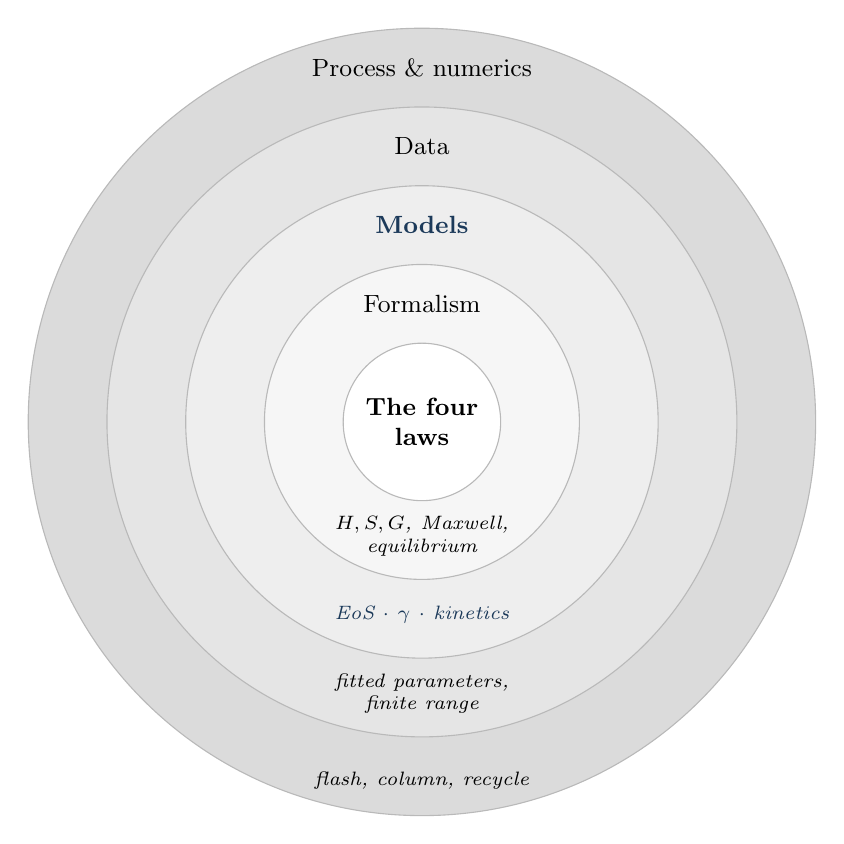
\begin{tikzpicture}[font=\sffamily]
  % Concentric shells: pristine (white) core out to empirical (grey) rim.
  \fill[gray!28,draw=gray!55] (0,0) circle (5cm);
  \fill[gray!20,draw=gray!55] (0,0) circle (4cm);
  \fill[gray!13,draw=gray!55] (0,0) circle (3cm);
  \fill[gray!7, draw=gray!55] (0,0) circle (2cm);
  \fill[white,  draw=gray!55] (0,0) circle (1cm);
  % Ring titles (upper band of each shell).
  \node[font=\bfseries\small,align=center] at (0,0)   {The four\\laws};
  \node[font=\small,align=center]          at (0,1.5) {Formalism};
  \node[font=\bfseries\small,text=accent]  at (0,2.5) {Models};
  \node[font=\small,align=center]          at (0,3.5) {Data};
  \node[font=\small,align=center]          at (0,4.5) {Process \& numerics};
  % Descriptors (lower band) so the map reads without the caption.
  \node[font=\scriptsize\itshape,align=center]         at (0,-1.45) {$H,S,G$, Maxwell,\\equilibrium};
  \node[font=\scriptsize\itshape,align=center,text=accent] at (0,-2.45) {EoS $\cdot$ $\gamma$ $\cdot$ kinetics};
  \node[font=\scriptsize\itshape,align=center]         at (0,-3.45) {fitted parameters,\\finite range};
  \node[font=\scriptsize\itshape,align=center]         at (0,-4.55) {flash, column, recycle};
\end{tikzpicture}
\caption{The layers of property prediction. The two inner shells follow from the
laws alone. The accent shell --- \emph{constitutive models} --- is the first
fault line: the laws say \emph{that} fugacities must match across phases, never
\emph{how} to compute one for a real mixture. From there outward, the theory is
necessary but no longer sufficient.}
\label{fig:bullseye}
\end{figure}

\begin{itemize}[leftmargin=1.4em,itemsep=2pt]
\item \textbf{The four laws (core).}\quad The zeroth, first, second and third
  laws define temperature, internal energy, entropy, and --- via Nernst --- an
  absolute zero of entropy. Parameter-free.
\item \textbf{Formalism.}\quad Pure manipulation yields the potentials $H$, $G$,
  $A$, the Maxwell relations, the equilibrium criteria (equality of fugacity
  across phases, $\Delta G=-RT\ln K$ for reaction) and the phase rule. Still
  derivable from nothing but the laws.
\item \textbf{Constitutive models --- where it first grips.}\quad The laws
  require fugacities to be equal across phases; they do not tell you how to
  \emph{compute} a fugacity for a real mixture. You must supply a model they do
  not give you --- an equation of state, an activity model, a kinetic law. In
  Choupo: \code{idealGas}/\code{SRK}/\code{PR}; \code{ideal}/\code{NRTL}/%
  \code{Wilson}/\code{UNIFAC}.
\item \textbf{Data --- ``go to the laboratory.''}\quad Those models carry
  parameters thermodynamics cannot predict: $T_c$, $P_c$, $\omega$, the Antoine
  constants, $C_p^\circ(T)$, $\Delta H_f^\circ$, $S^\circ$, the NRTL $a_{ij}$.
  Each is measured or estimated, and each has a finite validity range. In
  Choupo, these are the \code{.dat} files.
\item \textbf{Process \& numerics.}\quad Where the predicted numbers are
  consumed --- flash, distillation, recycle --- and grip a second time, now
  numerically (multiple EoS roots, phase stability, initialisation).
\end{itemize}

\begin{keyidea}
Sommerfeld's difficulty is this picture: a theory that \emph{looks} axiomatic to
the rim, but stops being self-sufficient at the accent shell. The honest move is
not to paper over the seam between rigorous derivation and fitted correlation ---
it is to show exactly where it runs.
\end{keyidea}

\subsection{Where the models came from --- a genealogy}\label{sec:genealogy}

The chain in \S\ref{ch:thermo-chain} shows there are exactly \emph{two} ways to
a fugacity in a mixture: through an equation of state ($\varphi$) or through an
activity coefficient ($\gamma$).  Each has its own lineage, and knowing them
explains why the model list looks the way it does --- and why it is a
\emph{list} at all rather than a single answer.

\paragraph{The equation-of-state line (1873 $\rightarrow$).}
Van der Waals wrote one equation for both phases, continuous through the
critical point: the first time liquid and gas were the same substance in one
formula.  Redlich--Kwong (1949) improved the attraction term; Soave (1972) made
it obey the vapour-pressure curve by introducing the acentric factor;
Peng--Robinson (1976) repaired the liquid density.  All four share one skeleton
--- repulsion plus attraction, with the parameters generated from $T_c, P_c,
\omega$ --- which is why adding a new cubic to Choupo touches \emph{no data
file}.  Then the molecular branch: Wertheim's association theory (1984) led to
SAFT (1989) and PC-SAFT (2001), where a molecule is a \emph{chain of segments}
and the parameters are $m, \sigma, \varepsilon/k$ instead of the critical
triad.  That is exactly why PC-SAFT extrapolates in temperature and density
where a cubic drifts --- and why it cannot borrow the cubic's parameters.

\paragraph{The activity-coefficient line (1964 $\rightarrow$).}
Regular-solution theory failed on polar mixtures.  Wilson (1964) introduced
\emph{local composition} --- the admission that a molecule does not see its
neighbours in bulk proportions --- but could not describe a liquid--liquid
split.  NRTL (Renon \& Prausnitz, 1968) added non-randomness and \emph{could}:
that is why an LLE case in this guide reaches for NRTL and not Wilson.
UNIQUAC (Abrams \& Prausnitz, 1975) split the excess Gibbs energy into a
combinatorial part (size and shape) and a residual part (energy).  UNIFAC
(Fredenslund, 1975) made UNIQUAC \emph{predictive} by decomposing molecules
into functional groups, so a pair never measured could still be estimated.
COSMO-RS (Klamt, 1995) and COSMO-SAC (Lin \& Sandler, 2002) went further and
replaced the group table with the molecule's own screening-charge surface from
a quantum calculation --- the first genuinely \emph{a priori} route to
$\gamma$, and the one that needs no binary datum at all.

\paragraph{The electrolyte line (1923 $\rightarrow$).}
Debye--H\"uckel derived the ionic atmosphere and is \emph{exact} in the dilute
limit --- and only there.  Davies (1962) stretched it empirically to a few
tenths molal.  Pitzer (1973) abandoned the pretence of derivation and wrote a
virial expansion in molality that holds to seawater and beyond.  Edwards
\emph{et al.}\ (1978) extended that expansion to \emph{molecular} solutes ---
dissolved $\mathrm{NH_3}$, $\mathrm{CO_2}$, $\mathrm{H_2S}$ --- which a
charge-only correlation cannot price at all, since $z = 0$ makes it return
$\gamma = 1$ identically.  eNRTL (Chen, 1982) carried local composition into
ionic solutions, which is what makes a mixed solvent --- salt plus water plus
ethanol --- tractable at all.

\paragraph{Choosing among the three aqueous models.}
The bench offers \code{davies}, \code{pitzerHMW} and \code{edwardsPitzer} as
the \code{activityModel} of a \code{speciate} operation, and they are not
interchangeable:

\begin{itemize}[leftmargin=1.4em,itemsep=2pt]
\item \code{davies} --- one line, no parameters, trustworthy to about
  $I \approx 0.5$ mol/kg and \emph{announced} as indicative beyond it.  Every
  neutral solute gets exactly $1$.  Use it for a first look and for teaching
  what a dilute correlation is.
\item \code{pitzerHMW} --- the Harvie--M\o ller--Weare parameterisation, per
  ion, with ternary mixing.  The right tool for brines, scaling and seawater.
\item \code{edwardsPitzer} --- a \emph{different} truncation of Pitzer's
  expansion, extended to molecules, and the one its
  $\mathrm{NH_3}/\mathrm{CO_2}/\mathrm{H_2S}/\mathrm{SO_2}$ parameters were
  regressed in.  Use it for weak-electrolyte and sour-water systems.
\end{itemize}

The last point generalises and is worth stating once: \textbf{a parameter set
belongs to the equation it was fitted in.}  Pitzer's expansion admits several
truncations, and a $\beta$ regressed under one of them is not a $\beta$ for
another.  Quoting a published number inside a different model is a category
error that no amount of agreement in one test case repairs, which is why
Choupo carries the two Pitzer engines side by side under distinct names
rather than merging their parameter tables.

\begin{keyidea}
Each model was invented because the previous one \emph{failed} at something
specific.  The list is not a menu of equivalent options; it is a history of
failures, each one repaired.  Choosing a property method is therefore choosing
\emph{which failure you can live with} in your system --- which is why this
architecture insists that the choice be declared in the case file, verified at
assembly, and confessed in the log.  A simulator that hides the choice behind a
dropdown has not removed the failure; it has removed your view of it.
\end{keyidea}

\subsection{The glass-box promise}

Because the outer shells are empirical, every number Choupo predicts should
travel with two things attached:

\begin{itemize}[leftmargin=1.4em,itemsep=2pt]
\item \textbf{Provenance} --- which method produced it (rigorous derivation,
  fitted correlation, or group-contribution estimate) and the source of each
  parameter (a measured datum or an estimate).
\item \textbf{Validity awareness} --- whether a correlation is \emph{extrapolating
  beyond its fitted range}, with a warning when it is, rather than a confident
  number where none is warranted.
\end{itemize}

\begin{intuition}
Ask Choupo for the vapour pressure of nitrogen at room temperature and it
\emph{refuses}: $\mathrm{N_2}$ is supercritical there (its critical temperature
is $-147\,$\textdegree C), and a saturation pressure does not exist above the
critical point. The $P^{\mathrm{sat}}$ curve simply \emph{breaks} at $T_c$
instead of extrapolating Antoine into a meaningless ${\sim}600\,$bar. That
refusal is the whole promise in miniature: the model declines to invent a number
the physics forbids.
\end{intuition}

\subsection{Where we are heading}

A single property over a wide temperature span is not one problem --- it is
several physical regimes stitched together, and your confidence in any predicted
number rises and collapses as you cross them. Figure~\ref{fig:ribbon} is the
destination of this guide: the vapour pressure of a
\textbf{water\,/\,ethanol\,/\,benzene} mixture from $-200$ to $1000\,$\textdegree C,
drawn not as a curve but as a band of \emph{confidence}.

\begin{figure}[h]
\centering
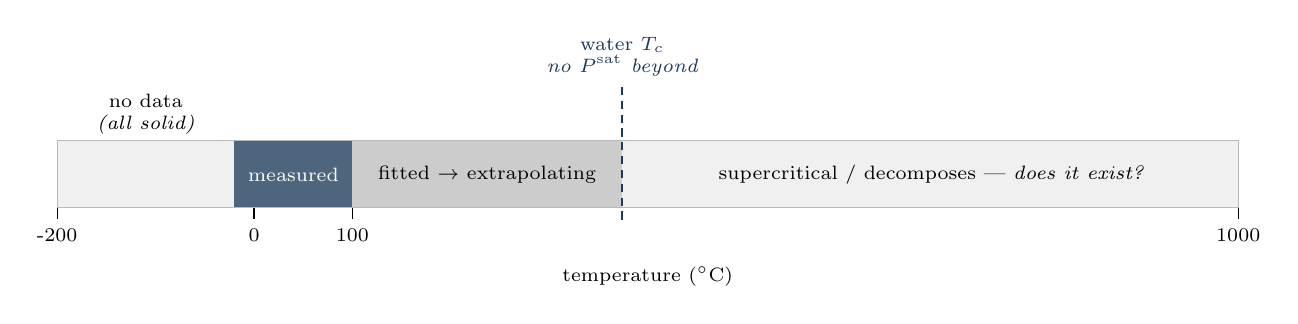
\begin{tikzpicture}[font=\sffamily]
  % x = (T + 200) * 0.0125  -> -200 maps to 0, +1000 maps to 15.
  \def\barh{0.85}
  \fill[gray!12]   (0,0)     rectangle (2.25,\barh);   % no data (cryogenic)
  \fill[accent!78] (2.25,0)  rectangle (3.75,\barh);   % measured
  \fill[gray!40]   (3.75,0)  rectangle (7.175,\barh);  % fitted -> extrapolating
  \fill[gray!12]   (7.175,0) rectangle (15,\barh);     % supercritical / decomposes
  \draw[gray!55]   (0,0) rectangle (15,\barh);
  % Band labels.
  \node[font=\scriptsize,align=center]          at (1.125,\barh+0.34) {no data\\\itshape(all solid)};
  \node[font=\scriptsize,text=white]            at (3.0,\barh/2)      {measured};
  \node[font=\scriptsize,align=center]          at (5.46,\barh/2)     {fitted $\rightarrow$ extrapolating};
  \node[font=\scriptsize,align=center]          at (11.1,\barh/2)     {supercritical / decomposes --- \itshape does it exist?};
  % Critical-temperature wall (where the property ceases to exist).
  \draw[densely dashed,accent,thick] (7.175,-0.15) -- (7.175,\barh+0.7);
  \node[font=\scriptsize,text=accent,align=center,above] at (7.175,\barh+0.7) {water $T_c$\\\itshape no $P^{\mathrm{sat}}$ beyond};
  % Temperature ticks.
  \foreach \t/\x in {-200/0, 0/2.5, 100/3.75, 1000/15} {
    \draw (\x,0) -- (\x,-0.14);
    \node[font=\scriptsize,below] at (\x,-0.14) {\t};
  }
  \node[font=\scriptsize,below] at (7.5,-0.62) {temperature ($^\circ$C)};
\end{tikzpicture}
\caption{The same property, five honesties. A narrow window where we actually
have data; degradation outward as the correlation extrapolates; a hard
\emph{wall} at the critical temperature where the property ceases to exist (the
nitrogen refusal, generalised); and a cryogenic desert where every species has
frozen solid (ethanol last, at $-114\,$\textdegree C) and there is simply no
data. The theory runs to both edges; reality and data do not.}
\label{fig:ribbon}
\end{figure}

We build each piece of that picture in the chapters that follow --- estimating a
missing component (\S\ref{ch:joback}), curating the mixture models against lab
points (\S\ref{ch:pairs}), and testing whether the data itself is even consistent
(\S\ref{ch:consistency-props}). We read that span regime by regime at the end of
this introduction (\S\ref{sec:span}), and return to solve it numerically, end to
end, at the close.

\subsection{Anatomy of a component: where the numbers come from}

Open any \code{.dat} and you see a flat list of numbers. The natural question ---
the one this whole guide turns on --- is: \emph{which of these are independent
inputs, and which derived properties does the engine actually build from them?}
Let us read \file{acetone.dat} field by field and follow each number to the
property it feeds and to the line of code that consumes it.

\begin{center}\footnotesize
\begin{tabularx}{\linewidth}{@{}l>{\raggedright\arraybackslash}X@{}}
\toprule
\textbf{Field} & \textbf{What it is, and what it builds} \\
\midrule
\multicolumn{2}{@{}l}{\itshape Identity} \\
\code{MW} & molar mass; converts molar $\leftrightarrow$ mass everywhere. \\
\addlinespace[2pt]
\multicolumn{2}{@{}l}{\itshape Caloric anchors --- \code{standardThermochemistry}} \\
\code{dHf\_298} $\Delta H_f^\circ$ & the \emph{position} of the enthalpy scale: bond energy $C_p$ knows nothing about (combustion calorimetry). \\
\code{s\_298} $S^\circ$ & the \emph{absolute} (third-law) entropy at 298\,K --- a true zero-referenced value, not a difference. \\
\addlinespace[2pt]
\multicolumn{2}{@{}l}{\itshape Caloric shape --- \code{idealGasHeatCapacity}} \\
\code{coefficients} $C_p^\circ(T)$ & the master correlation: integrated to give the \emph{temperature shape} of $H$, $S$, $G$ (below). \\
\addlinespace[2pt]
\multicolumn{2}{@{}l}{\itshape Corresponding-states trio} \\
\code{Tc}, \code{Pc} & critical point: set the \emph{size} of the cubic-EoS attraction term $a_c$, and the reduced temperature $T_r=T/T_c$. \\
\code{omega} $\omega$ & acentric factor: sets the \emph{temperature shape} of that attraction, $\alpha(T_r;\omega)$ --- how non-spherical / polar the molecule is. \\
\addlinespace[2pt]
\multicolumn{2}{@{}l}{\itshape Phase change} \\
\code{Tb}, \code{HvapTb} & boiling point + latent heat at $T_b$; with \code{Tc} drive Watson's $\Delta H_{\mathrm{vap}}(T)$. \\
\code{Vliq} & liquid molar volume (Poynting, liquid density). \\
\addlinespace[2pt]
\multicolumn{2}{@{}l}{\itshape Correlations \& recipes} \\
\code{vaporPressure} & Antoine $\log_{10}P^{\mathrm{sat}}=A-B/(T+C)$, with its \code{Trange}; the saturation curve. \\
\code{groups} & the molecular decomposition a group-contribution estimator / UNIFAC reads (the curation recipe, \S\ref{ch:joback}). \\
\code{diffusionVolume} & Fuller gas diffusivity $\Rightarrow$ Lewis number (wet-bulb). \\
\bottomrule
\end{tabularx}
\end{center}

\subsubsection*{The caloric engine: \texorpdfstring{$H$, $S$, $G$}{H, S, G} from \texorpdfstring{$C_p$}{Cp}}

This is the mechanism behind ``other properties that derive from here'' --- and
it is worth seeing \emph{how one arrives at $S(T)$}, since that is the step that
trips everyone up. Start from the laws, at constant pressure. Heat capacity
\emph{is} the temperature slope of enthalpy, $C_p=(\partial H/\partial T)_P$, so
\[
dH = C_p\,dT.
\]
For entropy, the second law gives $dS=\delta q_{\mathrm{rev}}/T$; at constant
pressure the reversible heat is $\delta q_{\mathrm{rev}}=C_p\,dT$, hence
\[
dS = \frac{C_p}{T}\,dT.
\]
That single step --- dividing by $T$ --- is the whole origin of the $\int C_p/T$.
Integrate each from a reference temperature and add the 298\,K anchor; Choupo
stores $C_p^\circ(T)$ and the two anchors (\emph{not} tables of $H$, $S$) and
evaluates:
\begin{align}
H^\circ(T) &= \underbrace{\Delta H_f^\circ}_{\text{position}} + \int_{298.15}^{T} C_p^\circ(T')\,dT'
   &&\text{\footnotesize(\code{Component::h\_pure\_ig}, \file{Component.cpp})}\\
S^\circ(T) &= \underbrace{S^\circ_{298}}_{\text{absolute}} + \int_{298.15}^{T} \frac{C_p^\circ(T')}{T'}\,dT'
   &&\text{\footnotesize(\code{Component::s\_pure\_ig})}\\
G^\circ(T) &= H^\circ(T) - T\,S^\circ(T)
\end{align}
For a mixture the engine adds the entropy of mixing $-R\sum y_i\ln y_i$ and the
pressure term $-R\ln(P/P_{\mathrm{ref}})$ (\code{ThermoPackage::S\_ig}). That is
the \emph{entire} ideal-gas caloric model --- no hidden tables.

These integrals are not done numerically. For a polynomial $C_p$ the primitive
is elementary --- it was solved \emph{once, on paper} --- so each call evaluates
a closed form,
\[
\int_{T_{ref}}^{T}\!\frac{C_p^\circ}{T'}\,dT'
   = a_0\ln\frac{T}{T_{ref}} + \sum_{k\geq1}\frac{a_k}{k}\bigl(T^k-T_{ref}^k\bigr),
\]
exact to machine precision in a handful of operations (\code{PolynomialCp::S}).
The standard correlations all share this property (NASA, Aly--Lee, Shomate have
closed primitives too); Choupo never runs a quadrature loop for $C_p$.

\begin{example}[Acetone $H$ and $S$ at 400\,K --- by hand, then by Choupo]
With $C_p^\circ(T)=6.301+0.2606\,T-1.253\!\times\!10^{-4}T^2+2.038\!\times\!10^{-8}T^3$
(units J\,mol$^{-1}$K$^{-1}$), integrating from 298.15 to 400\,K:
\[
\int C_p^\circ\,dT' = 8431~\text{J/mol},\qquad
\int \frac{C_p^\circ}{T'}\,dT' = 24.19~\text{J/(mol·K)}.
\]
So $H^\circ(400)=-217100+8431=\mathbf{-208669}$~J/mol and
$S^\circ(400)=295.30+24.19=\mathbf{319.49}$~J/(mol·K). Running
\code{choupoProps} on a one-point scan returns exactly
$H_{\mathrm{ig}}=-208669$~J/mol, $S_{\mathrm{ig}}=319.49$~J/(mol·K). The number
on the page is the number in the code --- and at 298.15\,K both integrals vanish,
so $H=\Delta H_f^\circ$ and $S=S^\circ_{298}$, the anchors laid bare.
\end{example}

\begin{keyidea}
$C_p$ gives the \emph{shape}; the formation values give the \emph{position}.
That is why the \code{.dat} lists $C_p^\circ(T)$ \emph{and} $\Delta H_f^\circ$,
$S^\circ$ separately --- not redundancy. And note the asymmetry: entropy has an
absolute zero for free (third law: $S\!\to\!0$ for a perfect crystal at
$T\!=\!0$), so $S^\circ_{298}$ is a genuine absolute; enthalpy has \emph{no}
natural zero, so $\Delta H_f^\circ$ must be \emph{measured} and supplied.
\end{keyidea}

\subsubsection*{What the critical properties and acentric factor actually do}

$T_c$, $P_c$, $\omega$ do nothing in the caloric equations above --- they enter
only when you ask for \emph{real-fluid} behaviour through a cubic equation of
state. There the attraction term is $a(T)=a_c\,\alpha(T_r)$, with $a_c$ fixed by
$T_c,P_c$ and the temperature shape fixed by $\omega$ (Soave/SRK):
\[
\alpha(T) = \bigl[\,1 + m(1-\sqrt{T_r})\,\bigr]^2,\quad
m = 0.48508 + 1.55171\,\omega - 0.15613\,\omega^2,\quad T_r=\tfrac{T}{T_c}
\]
(\code{SRK.cpp}; Peng--Robinson uses the analogous $\kappa(\omega)$). This
$a(T)$ is what produces the departure functions $H-H^\circ$, $S-S^\circ$ and the
compressibility $Z$ --- the real-gas correction layered on top of the ideal-gas
caloric result. The same $T_c,T_b$ also drive Watson's latent heat,
$\Delta H_{\mathrm{vap}}(T)=\Delta H_{\mathrm{vap}}(T_b)\,
[(T_c-T)/(T_c-T_b)]^{0.38}$ (\code{Component.cpp}).

\begin{intuition}
So why does \file{acetone.dat} carry $\omega$ at all if you are running the
default \code{idealGas}? Because the data is \emph{model-agnostic} and the model
decides which fields wake up. Under \code{idealGas} there is no departure, and
$\omega,T_c,P_c$ are simply never read. Select \code{SRK} for a high-pressure
compressor and the very same numbers come alive. The \code{.dat} is the
laboratory record; the model is the question you ask of it.
\end{intuition}

\subsubsection*{The entropy ledger, completed and verified}

The real-fluid entropy the isentropic machines consume is the
ideal-gas assembly above plus the model's departure,
\[
S(T,P,y) \;=\; S^{\mathrm{ig}}(T,P,y) \;+\; S^{\mathrm{R}}(T,P,y),
\]
with $S^{\mathrm{R}}$ supplied by whichever equation of state the case
declares: SRK carries the closed form
$S^{\mathrm{R}} = R\ln(Z-B) + (\mathrm{d}a/\mathrm{d}T / b)\,
\ln\!\bigl((Z+B)/Z\bigr)$ (Sandler's eq.~6.4-31, cited in
\file{SRK.cpp}), Peng--Robinson its generalised-cubic analogue, and
IF97 water evaluates its own fundamental-equation entropy directly.
One convention divergence is on record rather than hidden: PC-SAFT's
\code{S\_residual} returns the constant-density $(T,\rho)$ residual
\emph{without} the $+R\ln Z$ conversion to the $(T,P)$ departure the
cubics use --- stated in its own source comment, flagged in
\file{docs/design/entropy-glass-box-trace.md}, and open until a
witnessed fix; no shipped tutorial prices an isentropic machine on
PC-SAFT today.  The phase-crossing legs of the pure-component chain
--- and why the vaporisation step at the $298$~K datum is \emph{not}
$\Delta H_{\mathrm{vap}}/T$ --- are derived in the Theory Guide's
chapter on integral properties.

The whole chain is pinned by a witness the reader can run:
\code{tutorials/props/molecular/entropy01\_air\_ledger} publishes
every line for air at $400$~K and $2$~bar --- $s^{\circ}_i(T)$ per
component, $S^{\mathrm{ig}}$, $S^{\mathrm{R}}$, $S$ --- and its golden
holds the re-addition pure~$+$~mixing~$+$~pressure to the engine's own
total.  The ``What is entropy?''\ EduTool page performs that
re-addition on screen from a live run of the same case.

And the ledger buys a price tag: the \code{exergy} bench operation
evaluates the physical exergy $b = (h - h_0) - T_0\,(s - s_0)$ from the
same $H$ and $S$ surfaces at a \emph{declared} dead state
(\code{deadState \{ T0; P0; \}} --- the environment is the case
author's fact, and a missing block refuses rather than assuming one).
Because only differences at fixed composition enter, the enthalpy
datum, the $s^{\circ}_{298}$ anchors, the mixing term and the reference
pressure all cancel: $b$ is datum-independent.  Witness
\code{exergy01\_air\_dead\_state} prices the same air state at
$2136.7$~J/mol and pins the structural zero ($b = 0$ at the dead state
itself, on both legs).  Chemical exergy is deliberately refused by
name: it needs a standard-environment model (Szargut) that is a curated
data decision, not a formula.

% Drawn from src/propertyOps/ExplainProperty.H:31-67 (scope, dictionary form,
% refusals) and src/propertyOps/ExplainProperty.cpp:138-159 (the round-off
% identity check that refuses); numbers from
% tutorials/props/molecular/entropy01_air_ledger/expected.
\subsection{The ledger, explained: \code{explainProperty}}

The witness above publishes the lines; \code{explainProperty} publishes
where each line \emph{came from}.  For one property at one \code{state}
(\code{S\_real}, \code{S\_ig}, \code{H\_real}, \code{H\_ig}) it lists every
term with the record field or engine call behind it --- the
$s^{\circ}_{298}$ or $\Delta H^{\circ}_{f}$ datum, the $\int C_p/T$ term
as the \emph{difference} of two engine calls, the mixing and pressure
lines, the EoS residual --- re-adds them, and checks the sum against the
engine.  It computes no thermodynamics of its own; a gap beyond
round-off refuses.  In
\code{entropy01\_air\_ledger} the \code{explainS} op re-adds air's
$S_{\mathrm{ig}}$ at $400$~K and $2$~bar, $203.068 + 4.273 - 5.763 =
201.578$~J/(mol\,K), \code{gap\_total} pinned at $0$; the \code{explainH}
twin has no mixing and no pressure line.  Refused by name: an unknown
property, a datum off the ideal-gas rung, and a state answered by a
\code{pureFluids \{\}} override, whose ledger is the release's own
equation.

\subsection{From \texorpdfstring{$G$}{G} to equilibrium: what \texorpdfstring{$\Delta G^\circ$}{dG0} is (and is not)}

The single most common confusion in this whole subject is $\Delta G^\circ$
versus $\Delta G$. It is worth settling once, because $G$ is what the reactors
minimise and it is built from exactly the $H$ and $S$ above.

\textbf{First, the $^\circ$.}\quad It means \emph{reference state} --- each
species pure, ideal gas, at $1$\,bar --- but \emph{at the reaction temperature}
$T$. It does \emph{not} mean ``at 298\,K.'' So $\Delta G^\circ=\Delta G^\circ(T)$
varies with temperature; $\Delta G^\circ(298)$ is just one point on a curve.

\textbf{Then, the two are not the same thing.}
\begin{itemize}[leftmargin=1.4em,itemsep=2pt]
\item $\Delta G^\circ$ is the Gibbs change if reactants $\rightarrow$ products
  with \emph{everything in its standard state}. It is a \emph{fixed number} --- a
  property of the reaction at $T$.
\item $\Delta G$ is the \emph{actual} Gibbs change at the real composition (the
  real partial pressures). It is the \emph{driving force}.
\end{itemize}
The reaction quotient $Q$ bridges them, and equilibrium is where the driving
force --- not the reference number --- vanishes:
\[
\Delta G = \Delta G^\circ + RT\ln Q,
\qquad
\Delta G = 0 \text{ at equilibrium} \;\Rightarrow\;
\boxed{\;\Delta G^\circ = -RT\ln K\;}
\]

\begin{keyidea}
At equilibrium it is $\Delta G$ that is zero, \emph{never} $\Delta G^\circ$.
$\Delta G^\circ$ stays fixed and merely sets \emph{where} the equilibrium sits
(the value of $K$); the system gets there by shifting $Q$ until $\Delta G=0$. And
$\Delta G^\circ>0$ does not mean ``no reaction'' --- it means $K<1$, i.e.\ partial
conversion. Only the sign and size of $K$ change.
\end{keyidea}

\textbf{Where the number comes from} --- straight back to the caloric engine:
\[
\Delta G^\circ(T) = \Delta H^\circ(T) - T\,\Delta S^\circ(T)
   = \sum_i \nu_i\, g_i^\circ(T),
\qquad g_i^\circ(T) = h^{\mathrm{ig}}_i(T) - T\,s^{\mathrm{ig}}_i(T).
\]
Note the subtlety that confuses everyone: $h^{\mathrm{ig}}$ carries the
\emph{formation} enthalpy ($\Delta H_f^\circ$, an elements datum) while
$s^{\mathrm{ig}}$ is the \emph{absolute} (third-law) entropy. Mixing the two
references looks wrong --- but it is exactly right, because in a \emph{balanced}
reaction the element contributions cancel through $\sum_i\nu_i$. That is precisely
why the \code{.dat} carries $\Delta H_f^\circ$ \emph{and} $S^\circ$ separately:
each plays a different role, and they combine correctly only across a balanced
stoichiometry (\code{Component::g\_pure\_ig}; consumed in
\code{PFR.cpp}/\code{CSTR.cpp} as $K=\exp(-\Delta G^\circ/RT)$ and in the Gibbs
reactor's direct $G$-minimisation).

\smallskip
\noindent\textbf{How $K$ moves with $T$ (Gibbs--Helmholtz).}\quad
$\Delta G^\circ(T)$ is not a frozen datum --- it has its own temperature law, and
that law is a workhorse relation worth knowing by name. Gibbs--Helmholtz states
$\left[\partial(G/T)/\partial T\right]_P = -H/T^2$; applied to
$\Delta G^\circ=-RT\ln K$ it collapses to the van~'t~Hoff equation,
\[
\boxed{\;\frac{d\ln K}{dT} = \frac{\Delta H^\circ}{RT^2}\;}
\]
which is just Le~Chatelier made quantitative: an exothermic reaction
($\Delta H^\circ<0$) has $K$ \emph{falling} as $T$ rises. In Choupo it doubles as
a glass-box self-check --- the $K(T)$ the reactors build from $g^\circ(T)$ at each
temperature must show exactly this slope, or the enthalpy and the equilibrium
constant are disagreeing with each other.

\begin{intuition}
These relations are not ornaments. Gibbs--Helmholtz is \emph{how the equilibrium
moves with temperature} (above); its sibling, the \textbf{Gibbs--Duhem} equation
$\sum_i x_i\,\mathrm{d}\ln\gamma_i = 0$ (constant $T,P$), says the activity
coefficients of a mixture are \emph{not independent}. That single constraint is
exactly why measured VLE data can be \emph{tested} for thermodynamic consistency
--- and why an activity model is built from one $G^{\mathrm{E}}$ function rather
than fitting each $\gamma_i$ freely. It is the engine of
\S\ref{ch:consistency-props}.
\end{intuition}

\subsection{A worked span: water\,/\,ethanol\,/\,benzene, \texorpdfstring{$-200$}{-200} to \texorpdfstring{$1000\,$\textdegree C}{1000 C}}
\label{sec:span}

Put the three together and sweep the temperature. This one mixture crosses
\emph{every} regime of property prediction, and is the honest way to see both how
properties are obtained \emph{and} where the models give out --- which is exactly
the colour band of Figure~\ref{fig:ribbon}, now read regime by regime. (Critical
temperatures: ethanol $241\,$\textdegree C, benzene $289\,$\textdegree C, water
$374\,$\textdegree C; melting points: ethanol $-114$, water $0$, benzene
$5.5\,$\textdegree C.)

\begin{center}\footnotesize
\begin{tabularx}{\linewidth}{@{}p{2.45cm}>{\raggedright\arraybackslash}X>{\raggedright\arraybackslash}X@{}}
\toprule
\textbf{Regime} & \textbf{How a property is obtained} & \textbf{Where the model gives out} \\
\midrule
$-200$ to $\sim0\,$\textdegree C \newline {\scriptsize solids (SLE)}
 & melting points $T_m$, $\Delta H_{\mathrm{fus}}$, solid $C_p$; freezing-point depression; sublimation $P^{\mathrm{sat}}$
 & \textbf{low-T edge.} Below every Antoine \code{Trange}: $P^{\mathrm{sat}}$ would extrapolate blindly. Solid-phase data is sparse --- a cryogenic \emph{data desert}. \\
\addlinespace
$\sim0$ to $\sim65\,$\textdegree C \newline {\scriptsize two liquids (LLE)}
 & activity model (\code{NRTL}/\code{UNIFAC}) for $\gamma$; water/benzene nearly immiscible, ethanol the cosolvent
 & VLE-fitted parameters do \emph{not} serve LLE; \code{Wilson} cannot represent a liquid split at all; without $T$-dependent parameters the miscibility gap appears/vanishes wrongly. \\
\addlinespace
$\sim65$ to $\sim100\,$\textdegree C \newline {\scriptsize boiling (VLLE)}
 & Antoine $P^{\mathrm{sat}}$ $+$ $\gamma$--$\phi$ $+$ three-phase flash (Gibbs minimisation); ethanol/water + ternary azeotrope ($\sim64.9\,$\textdegree C)
 & azeotrope sensitivity --- a small $\gamma$ error moves the column design; bubble-point (Wang--Henke) distillation is unstable \emph{through} an azeotrope (use \code{model simultaneous}). \\
\addlinespace
$\sim100$ to $\sim290\,$\textdegree C \newline {\scriptsize vapour $\to$ near-critical}
 & cubic EoS (\code{SRK}/\code{PR}) with $k_{ij}$; departure functions $H-H^\circ$, $S-S^\circ$, $Z$
 & cubics degrade as the critical region is approached; $k_{ij}$ often needs to be made temperature-dependent over so wide a span. \\
\addlinespace
$\sim290$ to $374\,$\textdegree C \newline {\scriptsize mixed super/sub-critical}
 & the method itself must switch $\gamma$--$\phi$ $\rightarrow$ $\phi$--$\phi$ (one EoS for every phase)
 & above a species' $T_c$ the activity-coefficient picture loses meaning; no single $\gamma$ model spans the switch; near-critical accuracy is poor. \\
\addlinespace
$374$ to $1000\,$\textdegree C \newline {\scriptsize supercritical $+$ reaction}
 & $\phi$--$\phi$ EoS; wide-range $C_p^\circ(T)$ for the caloric terms
 & \textbf{high-T edge.} $P^{\mathrm{sat}}$ ceases to exist above $T_c$ (Choupo \emph{refuses} it, \S1.2); and the species thermally \emph{decompose} --- the fixed-component assumption fails: do they still exist? \\
\bottomrule
\end{tabularx}
\end{center}

The two edges --- the ones you asked to watch --- fail for opposite reasons but
teach the same lesson. At the \textbf{cold edge} there is simply no data: every
correlation is fitted to a window that starts well above $73\,$K, the species are
frozen, and a confident number there would be invention, not prediction. At the
\textbf{hot edge} the theory keeps producing numbers --- Antoine will gladly
report a vapour pressure at $800\,$\textdegree C --- but the \emph{physics} has
moved on: past each $T_c$ no saturation exists, and past a few hundred degrees
the molecules are no longer the molecules in the \code{.dat}. In both cases the
correct output is a \emph{flag}, not a figure.

\begin{pitfall}
No single model spans this axis. A run that quietly uses one $\gamma$ model and
one cubic from $-200$ to $1000\,$\textdegree C is not ``general'' --- it is
extrapolating through three regime changes in silence. The wide span is not one
problem; it is five problems wearing one temperature axis.
\end{pitfall}

\begin{intuition}
What Choupo ships \emph{today} covers the middle of this span honestly: cubic
EoS, \code{ideal}/\code{NRTL}/\code{Wilson}/\code{UNIFAC} activity, Antoine
$P^{\mathrm{sat}}$, Watson $\Delta H_{\mathrm{vap}}$, three-phase VLLE by Gibbs
minimisation, and azeotropic columns via the simultaneous MESH solver.  Since
2026-08-03 it also carries PC-SAFT with Wertheim association (the 2B and 4C
schemes; Theory Guide, the PC-SAFT chapter) for the hydrogen-bonding
non-ideality, and the electrolyte engines --- Pitzer, eNRTL, the
Harvie--M{\o}ller--Weare and Edwards truncations --- for the ionic edge.  What it
does \emph{not} carry is a wide-range near-critical package, and no
association or electrolyte model here is a general-purpose black box: each
is declared by the case, announced by the run, and parameterised from a cited
record.  So for the near-critical edge, and for any mixture the curated
parameters do not reach, Choupo's job is not to fake accuracy it does not
have --- it is to predict where it can and to \emph{say so} where it cannot.
That honesty is the product.
%  This box used to say Choupo carried NO association and NO electrolyte
%  models; both had shipped before the 2026-09-03 coverage sweep read it
%  back (CLAUDE.md §10: bury the absence you just filled).
\end{intuition}

% Drawn from src/propertyOps/FreezingPoint.H:31-60 (the equality, the bracket,
% the refusal, the diagnostics) and src/propertyOps/FreezingPoint.cpp:72-87,
% 110-118, 134-140; numbers from
% tutorials/props/electrolyte/fpd01_nacl_freezing/system/propsDict and
% tutorials/props/electrolyte/fpd01_nacl_freezing/expected.
\subsection{The low-\texorpdfstring{$T$}{T} edge on a real case: \code{freezingPoint}}

The solid row above, on a case.  \code{freezingPoint} traces the
freezing-point curve $T_f(m)$ of a single salt in water as
chemical-potential equality between ice and the solution's water,
\[
   f_{\mathrm{solid}}(T) \;=\; a_w(m,T)\,P^{\mathrm{sat}}(T),
\]
the left side an actual crystallising \code{SolidPhase}, the right the
Pitzer salt surface's water activity.  Routing through the phase makes
its refusals (no $\Delta H_{\mathrm{fus}}$, no triple point) and its
announced approximations (the neglected heat-capacity term, the
sub-freezing $P^{\mathrm{sat}}$ extrapolation) fire on a real run.  It
publishes the curve, $T_f$ and the depression at the grid end, the
dilute-limit slope against $\nu K_f$ (water's \emph{derived} cryoscopic
constant) and the AAD against a \code{validation} dataset.  A grid point
whose bracket holds no root is refused by name --- a eutectic the
single-salt model does not contain.  Witness \code{fpd01\_nacl\_freezing}:
NaCl to $2.0$~mol/kg, $T_f = 266.325$~K there (depression $6.835$~K),
slope$/\nu K_f = 0.931$, one interim measured point (AAD $0.046$\,\%).

% =====================================================================
\section{The Choupo property architecture --- the complete map}
\label{ch:architecture}

Everything in this guide hangs off one architecture.  This chapter is the
complete map, stated once; every later chapter is a room in this house.

\subsection{The flow}

\begin{quote}
\texttt{constant/thermoPhysPropDict} \emph{declares} $\;\rightarrow\;$ the builder
\emph{loads, verifies and announces} (it never estimates) $\;\rightarrow\;$ the
engine \emph{computes} $\;\rightarrow\;$ the run log \emph{confesses}.
\end{quote}

Estimation is a curation-time act (the props bench writes a reviewable
\texttt{.dat}); assembly-time refusal is loud (a missing declared parameter
file, a $k_{ij}$ regressed for another cubic, a vapour method the liquid path
cannot serve).  The log then shows the whole assembly: the VLE world, the
reference rung of every group, and every pair parameter with its source file.

\subsection{The grammar --- the axes of a property package}

\begin{center}
\small
\begin{tabular}{@{}llp{6.6cm}@{}}
\toprule
\textbf{Axis} & \textbf{Slot} & \textbf{What it fixes}\\
\midrule
components & \texttt{components ( ... )} & identity; a salt's \texttt{dissociatesTo} names its ions\\
phases & \texttt{phases}; the component's own \texttt{solidPhases\{\}} block & which phases exist; $\rho_p$, $k_v$ for solids (retired \texttt{phases/solid/} kept as a legacy read only)\\
model per PHASE & \texttt{equilibrium \{ formulation ...; liquid \{...\} vapour \{...\} \}} & ONE Gibbs surface per phase --- the \texttt{formulation} selects the VLE world\\
convention per GROUP & reference rungs (\texttt{referenceBasis}) & renormalisations of one surface: solvent on Raoult, solutes on Henry, ions on aqueous infinite dilution\\
correlation per COMPONENT & the component \texttt{.dat} (+ overrides) & pure-species data; legal for transport and pure correlations, never for the equilibrium surface\\
parameter per PAIR & \texttt{parameters \{ ...Pairs \{...\} \}} & declared FILE, verified at assembly, cited to its source\\
mixing per PROPERTY $\times$ PHASE & \texttt{mixing} slots + \texttt{effective\{\}} & how pures combine (Wilke, Grunberg--Nissan, van-der-Waals one-fluid); two-phase closures (a suspension's Thomas/Einstein viscosity) live in \texttt{effective\{\}}, because they are \emph{media closures}, not thermodynamic mixing\\
chemistry & \texttt{chemistry \{ salts (...); \}} & real equilibria with $K(T)$ and $\Delta H$\\
package per UNIT & unit \texttt{thermo \{\}} & the spatial axis: a unit selects ANOTHER whole package --- never a partial patch of single axes (that is the road to two surfaces in one phase); the model boundary is audited ($\Delta H$ at the seam)\\
phase equilibrium & \texttt{phaseEquilibrium \{\}} & for each coexisting phase pair, the imposed equality and the COMMON DATUM (e.g. \texttt{link muEquality; datum aqueousInfDil; transfer <pair-file>;}) --- the bridge between surfaces, first-class and declared, never implicit\\
\bottomrule
\end{tabular}
\end{center}

Provenance is an \emph{attribute of every value}, not an axis: each resolved
number carries a quality word
(\texttt{measured > fitted > correspondingStates > estimated > asserted}),
and an \texttt{asserted} value --- a pinned constant, a user polynomial, a user
table --- is refused without its written \texttt{why}.

\subsection{The five formulations}

A case declares one \code{equilibrium.formulation}; the builder assembles that
one natively and gives every other shape a named refusal.  Each is validated
against measured data in this guide:
\begin{center}
\small
\begin{tabular}{@{}llll@{}}
\toprule
\textbf{Formulation} & \textbf{Liquid method} & \textbf{K-value} & \textbf{Natural home}\\
\midrule
\texttt{gammaPhi} & \texttt{activity.NRTL} (Wilson, UNIQUAC, UNIFAC, cosmoSAC) & $\gamma_i P^{sat}_i/P$ & organic mixtures\\
\texttt{gammaGamma} & one activity model \emph{per named liquid phase} & $\gamma^{\alpha}_i/\gamma^{\beta}_i$ & LLE / VLLE, extraction\\
\texttt{diluteSolution} & \texttt{solution.henryDilute} & $\gamma^*_i H_i/P$ & dissolved gases\\
\texttt{phiPhi} & \texttt{eos.SRK} / \texttt{eos.PengRobinson} / \texttt{PCSAFT} & $\varphi^L_i/\varphi^V_i$ & high pressure, near-critical\\
\texttt{electrolyteGammaPhi} & \texttt{Pitzer} / \texttt{eNRTL} (molality) & ion activities, osmotic & brines, salts, mixed solvent\\
\bottomrule
\end{tabular}
\end{center}

\noindent\texttt{gammaGamma} is the one that surprises people: two coexisting
liquids are \emph{two phases}, each entitled to its own Gibbs surface, and the
split is found by minimising $G$ directly rather than by iterating $K$ --- a
symmetric $\gamma$-model would otherwise collapse onto the trivial $K=1$
saddle.  That is the legality rule of \S\ref{ch:thermo-chain} doing visible
work.

\subsection{The five component routes}

\begin{enumerate}
\item \textbf{Standard, by name} --- \texttt{data/standards/components/}
      (exact-name $O(1)$, every value cited, the engine refuses to write there).
\item \textbf{Local, by name} --- \texttt{data/local/components/} is the
      \emph{private} working tier (gitignored; shipped empty).  Records are
      runtime-usable, but every use is announced as
      \texttt{[local] UNVERIFIED}; a local record never shadows a standard
      one.  Integrity and provenance gates make a local record inspectable,
      not automatically authoritative.
\item \textbf{New, defined in the case} --- \texttt{myCase/constant/components/}:
      a new molecule (estimated and labelled), a new ion, a pseudo-component
      lump.  The case runs self-contained from day one; promotion into the
      standards tree is a \emph{requested, reviewed curation act} after
      validation.
\item \textbf{Standard + overlay} --- a partial case file merges field-by-field
      over the standard entry (sample-specific measured data, a new model
      block); the run announces the merge.
\item \textbf{Solids} --- solid reference rungs, solids on their own stream
      channel, and the iron rule: a dissolving salt's solid formation enthalpy
      is ION-DERIVED ($H_f^{solid}=\sum\nu_i h_{f,aq,i}-\Delta H_{soln}$),
      never a stored duplicate.
\end{enumerate}

Thus component resolution is \textbf{case-local overlay $>$ standard $>$
local (private, announced)}.  This is an evidence ladder, not merely a search
path: moving a file up the ladder requires review and validation, not a
rename.

\subsection{The ChemSep import route}

The ChemSep 8.3 importer (\texttt{bin/curate/chemsep\_to\_choupo.py}) is
deliberately reproducible and reviewable.  It runs CAS-based de-duplication
against the standard catalogue, then a structural/provenance audit and an
internal $P^{\mathrm{sat}}(T_b)$ closure check on every imported component
record --- a closure check on the imported constants and predictive
correlation, not an independent comparison with laboratory data.

The same import stages NRTL, UNIQUAC and Wilson binary-pair records, each
passing identity, direction, licence, source-digest and exact unit-conversion
checks.  Their source does not provide a captured temperature-validity range,
so they remain screening data and the runtime prints
\texttt{[local] UNVERIFIED} when one is selected.  Pair resolution is
\textbf{case-local/inline $>$ standard $>$ local $>$ announced ideal
default}; local data can therefore extend a case without silently changing
an approved standard.

The source boundary is intentional.  The unmodified third-party database and
its Artistic-2.0 licence are kept under \texttt{thirdParty/chemsep/}
(gitignored); the normalised, attributed records are written to the
\emph{private} \texttt{data/local/} tier --- they are never redistributed
with the public repository.  Literature values retain literature provenance;
Ambrose--Walton and other closures retain predictive provenance.  Missing
$C_p$, formation, electrolyte, adsorption, kinetic or transport data are not
inferred merely to make a record look complete.

The case additionally owns its \emph{equipment physics}: reaction kinetics in
\texttt{constant/reactions} (the heat of reaction always computed from the
formation datum and announced), per-machine measured curves (a dryer's
falling-rate data) in the unit's own folder, all inherited through the LOUD
fractal cascade (plant $\to$ sector $\to$ unit).

\subsection{The reference case}

The whole architecture is exercised by one designed flagship,
\texttt{tutorials/plant/lithiumBrinePlant} (under construction): salar brine
through Pitzer ponds and crystallisers, NF membrane Mg/Li separation,
solvent extraction with a student-defined extractant (the $\gamma$--$\varphi$
world and the audited Pitzer$\leftrightarrow$NRTL seam), electrodialysis,
60-bar CO$_2$ carbonation (the $\varphi$--$\varphi$ override and the Henry
world), a radical-kinetics burner satellite for thermal NO$_x$, batch
recrystallisation recipes, a control satellite, and the full outer ring
(fitting, sweeps, optimisation, sizing, costing, economics).  Later chapters
refer to its sectors by name.

\subsection{The principle}

No silent crutch, anywhere: every value is cited, estimated-and-labelled,
overlaid-and-announced, or asserted-with-a-why --- and the run log is where the
whole assembly confesses.  There is no ultimate model; hunting with the cat is
honest engineering, hiding the cat is fraud.

\section{The thermodynamic chain: how every equation here is
derived}\label{ch:thermo-chain}
% =====================================================================

Every K-value, activity coefficient and Henry constant in this guide falls
out of ONE chain of ideas.  This section walks it once, so that no equation
below ever has to be taken on faith.  (Full derivations: the Theory Guide,
chapters on flash, activity models, electrolytes and Henry's law.)

\subsection{1. Equilibrium is a Gibbs minimum}
The second law says an isolated system maximises entropy; recast at the
conditions a process engineer actually controls --- fixed $T$ and $P$ --- it
says a system minimises its \textbf{Gibbs energy} $G$.  For a multicomponent,
multiphase system,
\[
   dG \;=\; -S\,dT + V\,dP + \sum_i \mu_i\,dn_i,
   \qquad
   \mu_i \equiv \left(\frac{\partial G}{\partial n_i}\right)_{T,P,n_{j\neq i}},
\]
and at the minimum, moving a mole of $i$ between phases must change nothing:
\[
   \boxed{\;\mu_i^\alpha = \mu_i^\beta\;}\quad\text{for every component, across
   every pair of phases.}
\]
That single boxed statement is ALL the physics; everything else is bookkeeping
to make it computable.

\subsection{2. Fugacity: the workable currency}
$\mu_i$ is awkward: its absolute value is unknowable and it dives to $-\infty$
as $x_i \to 0$.  Lewis (1901) defined the \textbf{fugacity} $f_i$ through
$\mu_i = \mu_i^\circ + RT\ln(f_i/f_i^\circ)$ --- an ``effective pressure''
that equals $y_iP$ in an ideal gas.  Because $\ln$ is monotonic, the
equilibrium condition becomes
\[
   \boxed{\;f_i^{\,\alpha} = f_i^{\,\beta}\;}
\]
--- equal fugacities, phase by phase, component by component.  Every VLE
``world'' in Choupo is just a different, self-consistent way of WRITING
$f_i$ for a phase.

\subsection{3. Two routes to a mixture fugacity}
\textbf{Route A --- an equation of state} (works for any phase the EoS can
represent).  Define the fugacity coefficient $\varphi_i \equiv f_i/(y_iP)$;
thermodynamics gives it exactly from the volumetric behaviour,
\[
   RT\ln\varphi_i \;=\; \int_V^{\infty}\!\!\left[\left(\frac{\partial
   P}{\partial n_i}\right)_{T,V,n_j}\!\! - \frac{RT}{V}\right] dV
   \;-\; RT\ln Z ,
\]
so ONE model of $P(T,V,\mathbf n)$ --- a cubic like SRK with its $a(T)$,
$b$ and the pair correction $k_{ij}$ --- yields $\varphi_i$ for BOTH the
vapour root and the liquid root of the same cubic.

\textbf{Route B --- an activity model} (liquids only).  Split the liquid
fugacity into a reference times a correction,
$f_i^L = \gamma_i\,x_i\,f_i^{\circ}$, where the \textbf{activity coefficient}
$\gamma_i$ comes from a model of the excess Gibbs energy
($G^E$: NRTL, UNIQUAC, Wilson, Pitzer, eNRTL) via
$RT\ln\gamma_i = \partial G^E/\partial n_i$.
The price of Route B is choosing the \textbf{reference} $f_i^\circ$ --- and
that choice is a CONVENTION, not physics:

\begin{center}
\begin{tabular}{lll}
\textbf{Convention} & \textbf{Reference $f_i^\circ$} & \textbf{Normalised so} \\[2pt]
symmetric (Raoult)   & pure liquid: $P^{\mathrm{sat}}_i$ ($\times\,\varphi_i^{sat}\cdot$Poynting at high $P$) & $\gamma_i \to 1$ as $x_i \to 1$ \\
unsymmetric (Henry)  & infinite dilution: $H_{i,\mathrm{solv}} = \lim_{x\to 0} f_i/x_i$ & $\gamma_i^{*} \to 1$ as $x_i \to 0$ \\
electrolyte (aqueous)& ion at infinite dilution, $\mathrm{H^+(aq)}=0$ datum & $\gamma_\pm \to 1$ as $m \to 0$ \\
\end{tabular}
\end{center}

A supercritical solute HAS no pure liquid, so its only definable anchor is
the Henry limit --- which is why dissolved H$_2$/N$_2$ take the unsymmetric
convention, never an Antoine curve extrapolated above $T_c$.

\subsection{4. One Gibbs surface per phase --- the legality rule}
Gibbs--Duhem, $\sum_i x_i\,d\ln\gamma_i = 0$ at constant $T,P$, ties every
component's $\gamma$ in a phase to every other's: they must all derive from
ONE $G^E$ (or one EoS) surface.  Hence the rule that governs Choupo's
\code{thermoPhysPropDict} grammar: \emph{models per phase; conventions per
component-group within the phase; correlations per component; parameters per
pair}.  Mixing two $\gamma$-models (or two cubics) in one phase violates
Gibbs--Duhem and is refused.  Mixing CONVENTIONS in one phase is legal ---
solvent symmetric, solutes unsymmetric --- because a convention only
renormalises the same surface.

\subsection{5. The four worlds' K-values, assembled}
Setting $f_i^L = f_i^V$ with each route/convention gives every K-value this
guide uses:
\[
\begin{array}{llll}
\textbf{world} & f_i^L & f_i^V & K_i = y_i/x_i \\[3pt]
\gamma\text{-}\varphi & \gamma_i x_i P^{\mathrm{sat}}_i & y_i\varphi_i P
  & \dfrac{\gamma_i\,P^{\mathrm{sat}}_i}{\varphi_i\,P} \\[8pt]
\text{Henry (KK/KI)} & \gamma_i^{*} x_i H_i(T)\,e^{\bar v_i^\infty(P-P_s)/RT}
  & y_i\varphi_i P
  & \dfrac{\gamma_i^{*} H_i\,\mathcal P}{\varphi_i P} \\[8pt]
\varphi\text{-}\varphi & x_i\varphi_i^{L}P & y_i\varphi_i^{V}P
  & \dfrac{\varphi_i^{L}}{\varphi_i^{V}} \\[8pt]
\text{electrolyte} & \multicolumn{3}{l}{\text{ion activities from Pitzer/eNRTL on the aqueous rung;}}\\
 & \multicolumn{3}{l}{\text{full speciation (mass action + charge balance) where the case demands it}}
\end{array}
\]
Each row is one \code{equilibrium.formulation}
(\code{gammaPhi}, \code{diluteSolution}, \code{phiPhi},
\code{electrolyteGammaPhi}); the run log announces which world is live.  All four
are validated in the tutorials against measured data --- van~Ness-consistent
VLE sets ($\gamma$-$\varphi$), Wiebe/Larson solubilities (Henry, $\sim$2\%),
the Stryjek N$_2$--CH$_4$ isotherm ($\varphi$-$\varphi$, $\sim$2\%), and the
Hamer--Wu / calorimetric electrolyte sets.

\begin{intuition}
The whole edifice is: $G$ minimum $\to$ equal $\mu$ $\to$ equal $f$ $\to$
pick HOW to write $f$ per phase (an EoS or a $G^E$ model + a reference
convention) $\to$ a K-value.  When an equation in this guide looks arbitrary,
walk it back up this chain --- it never is.
\end{intuition}

% Drawn from src/propertyOps/MixingRules.H:31-71 (the rule, the ledger source,
% the refusals) and src/propertyOps/MixingRules.cpp:112-121 (the re-addition
% check); numbers from tutorials/props/molecular/mixrules01_natural_gas/expected.
\subsection{Route A, decomposed: \code{mixingRules}}

A cubic prices a mixture through two numbers, and the one-fluid rule
builds them from $n$ pures and $n(n-1)/2$ binary corrections:
\[
   a_{\mathrm{mix}}(T)=\sum_i\sum_j y_i\,y_j\,(1-k_{ij})\sqrt{a_i a_j},
   \qquad b_{\mathrm{mix}}=\sum_i y_i\,b_i .
\]
\code{mixingRules} publishes that decomposition at one \code{state}:
every pure $a_i(T)$ and $b_i$, every $k_{ij}$ as constructed, every pair's
term, and the identity that re-adds them to the $a_{\mathrm{mix}}$ the
engine runs.  The numbers come from \code{EquationOfState::mixingLedger},
a window on the \emph{same} \code{buildMix} the hot path runs --- the op
transcribes no rule of its own, and a re-addition gap beyond round-off
refuses.  Witness \code{mixrules01\_natural\_gas} (CH$_4$/N$_2$/CO$_2$,
$250$~K): one declared $k_{ij}$ (N$_2$--CH$_4$, $0.0289$) beside two pairs
on the announced $k_{ij}=0$ default; $a_{\mathrm{mix}}$ and
$b_{\mathrm{mix}}$ identical at $30$ and $1$~bar while $Z$ moves from
$0.9967$ to $0.9010$.  Refused by name: no equation-of-state slot, or a
model with no one-fluid rule --- ideal gas has no $a$, PC-SAFT mixes
inside its dispersion sum.

% Drawn from src/propertyOps/PhaseEnvelope.H:28-80 (purpose, geometry, what is
% not closed, the shared saturation solves) and
% src/propertyOps/PhaseEnvelope.cpp:118-140 (the root-jump test), 242-262 (the
% bracketed cricondentherm), 285-299 (a branch that never started); numbers
% from tutorials/props/molecular/envelope01_natural_gas/expected and
% tutorials/props/molecular/envelope02_root_jump/expected.
\subsection{The K-values, traced: \code{phaseEnvelope}}

\code{phaseEnvelope} draws the $P$--$T$ envelope of a mixture at fixed
feed \code{composition}: the bubble curve ($V/F \to 0$) and the dew curve
($V/F \to 1$), marched in \code{pressure}, written as CSV.
The saturation solves are \code{BubblePoint::compute} and
\code{DewPoint::compute}, the \code{bubbleT}/\code{dewT} units' own
routines.  The cricondentherm and the retrograde region live at the
nose, exactly where a single-specification march dies, so the op does
\emph{not} pretend to close the nose: each branch is traced while its
specification stays single-valued, and the last point is a stopping
point, never an extremum.  An \emph{interior} temperature maximum is
reported as a \emph{bracketed} cricondentherm; a converged point
discontinuous with its branch (a root jump) ends the branch.  Witnesses:
\code{envelope01\_natural\_gas} ($40$ dew points, cricondentherm
bracketed at $274.705$~K, bubble branch never started) and
\code{envelope02\_root\_jump} (bubble stopped at $18$~bar, dew at
$26$~bar).  Michelsen's arc-length continuation is the named,
unimplemented next step.

% =====================================================================
\section{Why a separate guide}
% =====================================================================

The Theory Guide answers \emph{how a model works} --- how a flash splits, how
an EoS predicts $Z$, how Levenberg--Marquardt minimises a residual.  This guide
answers a question that comes \emph{before} that: \emph{where do the numbers
that feed the models come from?}  A simulation is only as good as the $T_c$,
the NRTL pair, the heat of formation it stands on, and those are not handed
down --- they are estimated, fitted, and tested.

Choupo treats that as a first-class phase with its own binary (\code{choupoProps})
and its own lifecycle:

\begin{quote}
\textbf{CREATE} a component (from groups) \;$\rightarrow$\; \textbf{CURATE} the
mixture models (fit pairs, test data, choose by evidence) \;$\rightarrow$\;
\textbf{WIRE} the flowsheet \;$\rightarrow$\; \textbf{SIMULATE}.
\end{quote}

A \code{propsDict} of \code{operations} drives the first two stages.  A case may
have \emph{no} \code{flowsheetDict} at all (a pure properties case --- the
compound bench), or carry one and use props to curate the thermo it will
simulate.  Same files, same engine; only the centre of the GUI differs.

\begin{intuition}
The usual reflex is to click a property method and trust a badge.  Choupo's
stance (the ``see, then decide'' principle) is the opposite: you make the
estimate or the fit \emph{visible} --- the group build-up, the model curve
against the lab points, the consistency residual --- and decide from the
evidence in front of you.  Estimation has error; the point is to see it.
\end{intuition}

% =====================================================================
\section{Where curated data lives, and how a case selects it}\label{ch:property-package}
% =====================================================================

You estimated a $T_c$, fitted an NRTL pair, tested a heat of solution.  Two
questions follow: \emph{where does that number land}, and \emph{how does a case
use it}?  Choupo's answer is \emph{declarative property packages with
OpenFOAM-like explicit files}.

A curated value lands in a glass-box \code{.dat} in a tree organised by
\emph{what kind of thing} it is --- the intrinsic property of one substance, the
parameter of a pair, the equilibrium of a reaction:

\begin{lstlisting}
data/standards/
  components/<name>.dat            intrinsic, one substance (Tc, Antoine, Cp)
                                   + dissociatesTo { Na 1; Cl 1; }  [salts]
  species/<name>.dat               one modelSpecies file per species
                                   (Na, Cl, CO2aq, O2): formula + charge +
                                   medium-tagged thermo; never fed to a flowsheet
  (a crystal phase lives in its COMPONENT's own solidPhases{} block:
   rho_p, k_v and the dissolution equilibrium of its own solid --
   the phases/solid/ directory is RETIRED, legacy read only)
  chemistry/<name>.dat             FLAT; an equilibrium: dissolution,
                                   speciation (recordType names the family)
  parameters/.../<i>-<j>.dat       a pair: NRTL, Pitzer, eNRTL
  (methods/ is RETIRED: the reference basis is a consequence of the
   declared formulation -- the one-knob rule)
  (the system is declared INLINE in the case's constant/thermoPhysPropDict
   -- THE CENTRE; there is no shared package catalogue)
\end{lstlisting}

The arity rule decides \emph{which} file: a number that ``stands alone with the
molecule'' (the $T_c$ of water) lives with the component; a number that needs
two names (an NRTL pair) cannot, and goes to \code{parameters/}.  The Developer
Guide (\emph{the thermophysical property architecture}) gives the full layout
and the eight data kinds.

\paragraph{Declaring the system.}  A case does not list loose models and
parameters.  It \emph{declares} its thermophysical system --- one record that
names the components, the formulation, and the parameter files the run needs
(active chemistry lives beside it in \file{constant/chemistryDict}):

\begin{lstlisting}
recordType    thermophysicalPropertySystem;
schemaVersion 2;

components ( water NaCl );          // NaCl's dissociatesTo names the ions

equilibrium
{
    formulation electrolyteGammaPhi;

    aqueous
    {
        solvent            water;
        apparentComponents ( NaCl );  // stream carries the salt; the model
        activityModel { model Pitzer; }        //   activates its ions
        compositionBasis molality;
    }

    vapour { fugacityModel idealGas; }
}
% Pitzer pairs resolve by (cation,anion) name from parameters/; declared
% binaryParameters/binaryInteractions files load from their `source` paths
% and refuse when missing.
\end{lstlisting}

The flow is one sentence: \textbf{\code{thermoPhysPropDict} declares,
\code{ThermoPackageBuilder} assembles, \code{ThermoPackage} computes.}  The
declaration is the recipe; the builder loads what it names and mounts the
runtime object the unit operations consume.  An ordinary molecular case is
the same record degenerate --- no dissociation, no chemistry, a
\code{gammaPhi} block with an NRTL or an EoS slot.

\begin{intuition}
The boundary you must respect: \emph{curation estimates, runtime does not}.  You
may estimate, fit, and derive at the props bench --- and you \emph{see} it
(\S\ref{ch:joback}, \S\ref{ch:pairs}).  Once a case runs, the builder only
\emph{loads} existing case, standard or local records; it never invents a
missing property.  For activity models, an unresolved binary pair may use the
documented ideal default, but that fallback is announced and appears in the
provenance.  A required record with no defined fallback stops the run with a
clear message.  So: estimate, look, promote --- and inspect every local or
defaulted rung used by the package.
\end{intuition}

% =====================================================================
\section{Creating a component: Joback group contribution}\label{ch:joback}
% =====================================================================

When a component is missing from the catalogue and from the literature, you can
\emph{estimate} its pure-component constants from its molecular structure ---
the groups it is built from.  Choupo implements the \textbf{Joback} method
(Joback \& Reid, 1987; tabulated in Poling, Prausnitz \& O'Connell, \emph{The
Properties of Gases and Liquids}, 5th ed.), the \code{estimateComponent}
property operation.

\subsection{The method}

Each first-order group contributes a tabulated increment.  Summing the
increments and substituting into Joback's correlations gives the constants
(with $n_A$ the total number of atoms):

\begin{align}
T_b      &= 198.2 + \textstyle\sum_i n_i\,\Delta T_{b,i} \\
T_c      &= T_b \,\big/\, \big(0.584 + 0.965\,\Sigma\Delta T_c - (\Sigma\Delta T_c)^2\big) \\
P_c      &= \big(0.113 + 0.0032\,n_A - \Sigma\Delta P_c\big)^{-2} \quad[\text{bar}] \\
V_c      &= 17.5 + \textstyle\sum_i n_i\,\Delta V_{c,i} \quad[\text{cm}^3/\text{mol}] \\
\Delta H_f^{\circ}(298) &= 68.29 + \textstyle\sum_i n_i\,\Delta H_{f,i} \quad[\text{kJ/mol, ideal gas}] \\
\Delta H_{\text{vap}}(T_b) &= 15.30 + \textstyle\sum_i n_i\,\Delta H_{v,i} \\
C_p^{\text{ig}}(T) &= (\Sigma a - 37.93) + (\Sigma b + 0.210)T
                    + (\Sigma c - 3.91\!\times\!10^{-4})T^2
                    + (\Sigma d + 2.06\!\times\!10^{-7})T^3 .
\end{align}

The acentric factor $\omega$ is \emph{not} a group sum; Choupo derives it from
$(T_b, T_c, P_c)$ by the Lee--Kesler correlation, with $T_{br}=T_b/T_c$ and
$P_c$ in atm:
\begin{equation}
   \omega = \frac{-\ln P_c - 5.97214 + 6.09648/T_{br} + 1.28862\ln T_{br} - 0.169347\,T_{br}^6}
                 {15.2518 - 15.6875/T_{br} - 13.4721\ln T_{br} + 0.43577\,T_{br}^6}.
\end{equation}

A few first-order group increments (Joback \& Reid; the full table is in the
code, \code{src/propertyOps/EstimateComponent.cpp}):
\begin{center}\small
\begin{tabular}{lrrrr}
\toprule
group & $\Delta T_b$ & $\Delta T_c$ & $\Delta P_c$ & $\Delta H_f$ (kJ/mol)\\
\midrule
$-$CH$_3$        & 23.58 & 0.0141 & $-0.0012$ & $-76.45$ \\
$>$CH$_2$        & 22.88 & 0.0189 & $\ \ 0.0000$ & $-20.64$ \\
$-$OH (alcohol)  & 92.88 & 0.0741 & $\ \ 0.0112$ & $-208.04$ \\
$>$C$=$O (ketone)& 76.75 & 0.0380 & $\ \ 0.0031$ & $-133.22$ \\
aromatic $=$CH$-$& 26.73 & 0.0082 & $\ \ 0.0011$ & $\ \ 2.09$ \\
\bottomrule
\end{tabular}
\end{center}

\subsection{The structure is identity: the \code{groups\{\}} block and \code{bin/estimate}}

The molecular structure belongs \emph{with the substance}, like the formula:
a component's \code{.dat} declares its groups once, method-keyed inside
one \code{groups\{\}} block,
\begin{lstlisting}
groups
{
    joback ( { group CH3; count 2; } { group ketone; count 1; } );
    unifac ( { group CH3; count 1; } { group CH3CO; count 1; } );
}
\end{lstlisting}
(one home for every decomposition --- Joback and UNIFAC are different
tables, so each method keys its own list), and estimation needs no case
at all:
\begin{lstlisting}
bin/estimate acetone            # case-local first, then the standard catalogue
bin/estimate path/to/new.dat    # or an explicit file
\end{lstlisting}
The command runs the Joback engine on the component's own groups, prints the
full glass-box build-up (each group's increment, the closure chain, deviations
against any \code{reference} block), and drops \emph{one} stable proposal ---
\code{<name>.estimated.dat} --- next to the source, for you to review and
promote by hand.  It never writes into the frozen \code{data/standards/} tree,
and the solver still refuses to estimate at run time: estimation is a
\emph{curation} act with a paper trail, not a silent fill-in.

The \code{estimateComponent} operation remains the pedagogical form --- declare
the groups inline in a \code{propsDict} when you want the estimate itself to be
the lesson, as in the worked example below.

\subsection{Worked example: acetone}

Acetone, $\mathrm{CH_3\!-\!CO\!-\!CH_3}$, decomposes into $2\times\code{CH3}$ and
$1\times\code{ketone}$.  The operation prints the build-up and validates against
a \code{reference} block:

\begin{center}\small
\begin{tabular}{lrrr}
\toprule
Property & Joback & Reference (NIST) & Dev. \\
\midrule
$T_b$   & 322.1\,K        & 329.2\,K  & $-2.2\%$ \\
$T_c$   & 500.6\,K        & 508.1\,K  & $-1.5\%$ \\
$P_c$   & 48.0\,bar       & 47.0\,bar & $+2.2\%$ \\
$V_c$   & 209.5\,cm$^3$/mol& 209\,cm$^3$/mol & $\approx 0$ \\
$\omega$& 0.295           & 0.307     & $-3.9\%$ \\
$\Delta H_f^{\circ}$ & $-217.8$\,kJ/mol & $-217.1$\,kJ/mol & $+0.3\%$ \\
\bottomrule
\end{tabular}
\end{center}

Within a few percent on the criticals and almost exact on $\Delta H_f$ --- and
you \emph{see} the error, because the reference sits beside the estimate.

\begin{intuition}
\textbf{Know the method's limits.}  Joback is weak on $T_b$ of strongly
hydrogen-bonding species (ethanol's $T_b$ comes out $\sim$14\,K low), and it
yields \emph{no} Antoine / vapour-pressure parameters --- those need a fit
(\S\ref{ch:pairs}) or a corresponding-states correlation, a separate step.  An
estimate is a starting point you then anchor to data, never a final answer.
\end{intuition}

\begin{tutoriallink}
\file{tutorials/props/estimate/estimate\_acetone} --- the example above, groups in,
validated estimate out.
\end{tutoriallink}

% =====================================================================
\section{Curating mixture models: fitting binary pairs}\label{ch:pairs}
% =====================================================================

A pure-component set is not enough for a mixture: the non-ideality lives in the
\emph{binary interactions} (NRTL, Wilson).  Those parameters are regressed
against experimental VLE data by Levenberg--Marquardt --- the \code{fitParameters}
operation.

\subsection{The activity-coefficient models}

For a binary, the \textbf{NRTL} model gives the liquid-phase activity
coefficients from three adjustable numbers per pair --- $\tau_{12},\tau_{21}$
(temperature-dependent) and the non-randomness $\alpha$:
\begin{equation}
   \tau_{ij} = a_{ij} + \frac{b_{ij}}{T}, \qquad G_{ij} = \exp(-\alpha\,\tau_{ij}),
\end{equation}
\begin{equation}
   \ln\gamma_1 = x_2^2\!\left[\tau_{21}\!\left(\frac{G_{21}}{x_1+x_2 G_{21}}\right)^{\!2}
   + \frac{\tau_{12}\,G_{12}}{\left(x_2+x_1 G_{12}\right)^2}\right],
\end{equation}
and $\ln\gamma_2$ by swapping the indices.  So a pair carries four fittable
coefficients $(a_{12},b_{12},a_{21},b_{21})$ plus a fixed $\alpha$ (often $0.3$).
\textbf{Wilson} is the two-parameter alternative,
\begin{equation}
   \ln\gamma_1 = -\ln(x_1+\Lambda_{12}x_2)
   + x_2\!\left[\frac{\Lambda_{12}}{x_1+\Lambda_{12}x_2}
   - \frac{\Lambda_{21}}{x_2+\Lambda_{21}x_1}\right],
\end{equation}
which cannot represent a liquid--liquid split (use NRTL when one is suspected).

\subsection{Predicting without pairs: COSMO-SAC}\label{sec:cosmosac}

NRTL and Wilson need a fitted pair --- somebody measured that binary.
\textbf{COSMO-SAC} is the predictive alternative: the activity coefficients
come from each compound's \emph{sigma profile} --- the histogram of screening
charge density over its molecular surface, from a quantum-chemical
calculation done \emph{once, elsewhere, at curation time} --- and no binary
parameter exists at all.  Choupo implements the 2002 variant (Lin \&
Sandler), following the NIST benchmark implementation, as a plain activity
model: same interface as NRTL, selected the same way.

A compound carries its profile in its own \file{.dat}, as one or more
\emph{named parameter sets} (a compound may carry profiles from several
public collections, each labelled with its source):

\begin{lstlisting}[language=dict]
cosmo
{
    VT2005            // set name = its source collection
    {
        variant       cosmoSAC2002;
        source        "Mullins et al., IECR 45 (2006) 4389";
        area          [-] 106.3;      // A^2
        volume        [-] 118.8;      // A^3
        sigmaProfile  ( ... );        // 51 points, -0.025..0.025 e/A^2
    }
}
\end{lstlisting}

The case selects the model and, when a compound carries more than one set,
names which one:

\begin{lstlisting}[language=dict]
activityModel { model cosmoSAC;  source VT2005; }
\end{lstlisting}

A compound with a single set needs no \code{source} (its lone set is the
default); a multi-set compound without one is a loud error, as is a missing
\code{cosmo} block or a set whose declared \code{variant} does not match the
implemented constants --- a profile is never silently combined with another
variant's parameters.  The standard catalogue ships VT2005 sets for 77
components.  Validation: a pure component gives $\ln\gamma = 0$ exactly, and
the implementation is cross-checked bit-for-bit against an independent code
on the same equations and profiles.  What Choupo deliberately does
\emph{not} do is generate profiles (that is quantum chemistry, a curation
act outside the simulator) or bulk-import thousands of compounds.  Reference
case: \file{tutorials/props/molecular/cosmoSAC01\_water\_ethanol}.

\subsection{The residual the fit minimises}

The measurable is the bubble temperature.  At a fixed pressure $P$ and liquid
composition $x$, the bubble point is the $T$ that closes modified Raoult,
\begin{equation}
   \sum_i x_i\,\gamma_i(x,T)\,P_i^{\text{sat}}(T) = P
   \label{eq:bubbleT}
\end{equation}
(a Newton-1D in $T$; $P_i^{\text{sat}}$ from Antoine).  Levenberg--Marquardt
then drives the pair coefficients $\theta=(a_{12},b_{12},a_{21},b_{21})$ to
minimise the sum of squared bubble-temperature residuals against the data,
\begin{equation}
   \min_{\theta}\ \sum_k \big[\,T_{\text{bub}}(x_k;\theta) - T_{k}^{\text{exp}}\,\big]^2 .
\end{equation}

\begin{intuition}
\textbf{A low residual is not a good fit.}  At a \emph{single} pressure
$\tau_{ij}=a_{ij}+b_{ij}/T$ is nearly linear in both $a_{ij}$ and $b_{ij}/T$
over the narrow $T$ range of one isotherm/isobar, so $a$ and $b$ are
\emph{correlated} --- many $(a,b)$ pairs fit equally well and the optimum is a
valley, not a point.  \code{fitParameters} forms $J^{\mathsf T}J$ at the optimum
and reports the parameter correlation + confidence intervals so you SEE this;
the Theory Guide's \emph{Levenberg--Marquardt} and \emph{What is fittable}
chapters derive the diagnostic.  Fit across pressures, or fix $b$, to break it.
\end{intuition}

\subsection{See, then decide: the model overlay}

Before fitting, look.  Declare one scan \code{operation} per candidate model
(ideal, NRTL, Wilson), emitting the $(x, T_{\text{bubble}}, y_{\text{eq}})$
trio, and an \code{experimental \{\}} entry that overlays them --- and, with a
\code{dataset}, draws the measured points on top.  The student sees which model
the data actually picks: for ethanol/water at 1\,atm the ideal curve misses the
azeotrope entirely while NRTL lands on it.

\begin{tutoriallink}
\file{tutorials/props/compare/compare\_vle\_etoh\_water} --- ideal vs.\ NRTL bubble/dew
curves overlaid with measured VLE points (Carey \& Lewis, 1932).
\end{tutoriallink}

\subsection{Fit, then promote}

When a model earns its keep, \code{fitParameters} regresses its coefficients to
the data and writes a proposal to
\file{constant/parameters/<model>/<pair>.fit-<date>.dat}.  Promotion is a
deliberate, visible act: you inspect the parity plot and the identifiability
statistics (confidence intervals, parameter correlation) the fit reports ---
never a ``good fit'' badge --- and copy the proposal into the case's
\code{constant/} when you trust it.

% =====================================================================
\section{Testing the data itself: consistency}\label{ch:consistency-props}
% =====================================================================

Before fitting a model \emph{to} data, test whether the data is even
thermodynamically consistent --- a fit to bad data is a polished wrong answer.
The \code{vleConsistency} operation does this in three steps.

\subsection{Step 1 --- activity coefficients straight from the data}

It does not assume a model.  From each measured $(x_1, y_1, T)$ at the run
pressure $P$, modified Raoult gives the activity coefficient of each component
directly:
\begin{equation}
   \gamma_i = \frac{y_i\,P}{x_i\,P_i^{\text{sat}}(T)},
   \qquad P_i^{\text{sat}}(T)\ \text{from Antoine}.
\end{equation}
These are \emph{experimental} $\gamma_i$ --- the test now asks whether they obey
thermodynamics.

\subsection{Step 2 --- the Gibbs--Duhem point test}

The Gibbs--Duhem equation is the constraint every real mixture must satisfy at
constant $T,P$:
\begin{equation}
   \sum_i x_i\,\mathrm{d}\ln\gamma_i = 0
   \quad\Longrightarrow\quad
   x_1\frac{\mathrm{d}\ln\gamma_1}{\mathrm{d}x_1}
   + x_2\frac{\mathrm{d}\ln\gamma_2}{\mathrm{d}x_1} = 0 \ \ (\text{binary}).
   \label{eq:gd}
\end{equation}
The operation evaluates the left-hand side at each interior point (central
differences in $x_1$) and reports its max and mean magnitude --- the
\emph{point residual}.  A consistent set keeps it near zero.  (Isobaric data
adds a small $-H^{\mathrm E}/RT^2 \cdot \mathrm{d}T/\mathrm{d}x$ term, dropped
here; stated as a caveat, not hidden.)

\subsection{Step 3 --- the Herington area test}

Integrate \eqref{eq:gd} across the whole composition range: for an isothermal
set Gibbs--Duhem forces the net area of $\ln(\gamma_1/\gamma_2)$ to vanish.
Herington's isobaric form compares that net area to the absolute area and
corrects for the boiling-range:
\begin{equation}
   D = 100\,\frac{\left|\displaystyle\int_0^1 \ln\dfrac{\gamma_1}{\gamma_2}\,\mathrm{d}x_1\right|}
                 {\displaystyle\int_0^1 \left|\ln\dfrac{\gamma_1}{\gamma_2}\right|\mathrm{d}x_1},
   \qquad
   J = 150\,\frac{T_{\max}-T_{\min}}{T_{\min}},
\end{equation}
(both integrals by the trapezoid rule over the sorted points).  The set
\textbf{passes} when $|D-J| < 10$.  The GUI's consistency card plots
$\ln\gamma_1,\ \ln\gamma_2$ and $\ln(\gamma_1/\gamma_2)$ vs $x_1$ with the net
area shaded --- you SEE the $\pm$ areas cancel, not just the number.

Finally the infinite-dilution coefficients $\gamma_1^\infty,\gamma_2^\infty$
(the dilute-end limits) are reported --- the most stringent point of any model
later fitted to the set.

\begin{tutoriallink}
\file{tutorials/props/compare/compare\_vle\_etoh\_water} --- the \code{vleConsistency} op
on the Carey--Lewis ethanol/water data (Herington $|D-J|=4.6<10$, PASS).
\end{tutoriallink}

% =====================================================================
\section{The bench beyond thermodynamics}
\label{ch:bench-beyond}
% =====================================================================

Two operations ship in the props bench whose subject is not a property
package at all: a catalyst pellet and a recorded step response.  They are
here because the bench already has the right shape --- a model, a declared
input, a published answer with its own verification beside it.

% Drawn from src/propertyOps/ThielePellet.H:31-110 (scope, the published
% columns, what the op does not do) and src/propertyOps/ThielePellet.cpp:249-262
% (the scope announced on every run), 424-440 (verification tolerances);
% numbers from tutorials/props/reactor/thiele01_sphere_first_order/expected and
% tutorials/props/reactor/thiele02_prater_temperature/expected.
\subsection{One pellet: \code{thielePellet}}

\code{thielePellet} resolves a \code{kind catalyst;} asset record and
its effective diffusivity, solves the isothermal first-order
intraparticle problem numerically, and \emph{verifies} the answer against
the closed form --- a run missing its declared \code{verification}
tolerances exits~1.  It publishes the field $c(r)/c_s$, the Thiele
modulus $\phi$ with the effectiveness factor $\eta$ it produces, the
Weisz--Prater observable $\eta\phi^2$ and the swept $\eta(\phi)$ family
over three geometries.  The physics lives in
\file{src/unitOperations/reactor/pellet/PelletDiffusion}, where the four
reactors that today assume $\eta = 1$ will reach it.  Witness
\code{thiele01\_sphere\_first\_order}: CO in a $3$~mm alumina sphere at
$573.15$~K with a teaching $k = 40$~s$^{-1}$ gives $\phi = 1.016$,
$\eta = 0.6657$, verified to $1.3\times10^{-6}$;
\code{thiele02\_prater\_temperature} adds Prater's temperature field
($\Delta T_{\mathrm{centre}} = 15.57$~K).  It never decides whether
diffusion matters in the reader's case: it announces its scope on every
run --- first order, one temperature, one pellet size, both
external films neglected --- and judges nothing.

% Drawn from src/propertyOps/ReactionCurve.H:31-195 (the surrogate, the rules
% and their primaries, the refusals, what it does not do) and
% src/propertyOps/ReactionCurve.cpp:468-480 (the regression), 596-623 (the
% unresolved dead time); settings from
% tutorials/ctrl/ctrl17_step_reaction_curve/system/propsDict.
\subsection{A recorded experiment: \code{reactionCurve}}

Open-loop identification off a trajectory somebody else recorded.
\code{reactionCurve} reads a \code{choupoCtrl} trajectory, a
\code{manipulated} column and a \code{measured} one, cuts it into step
segments and fits each to the first-order-plus-dead-time surrogate
\[
   y(t) = y_0 + K\,\Delta u\left[1 - e^{-(t - t_{\mathrm{step}} - \theta)/\tau}\right],
   \qquad t \ge t_{\mathrm{step}} + \theta,
\]
by Nelder--Mead, then applies the named rules (\code{zieglerNichols},
\code{cohenCoon}, \code{imcLambda}).  It solves no plant: a missing
trajectory refuses.  It publishes $(K, \tau, \theta)$
with the fit's residual, plus segment, curve and tuning CSVs.  A segment that has not settled under the declared \code{settling}
test yields no time constant; a dead time within the sampling interval is
unresolved, and every rule dividing by $\theta$ is refused by name (IMC
never does).  Witness
\file{tutorials/ctrl/ctrl17\_step\_reaction\_curve} (a \code{ctrl} case,
run first): the composition loop takes all three rules; the temperature
loop refuses Ziegler--Nichols and Cohen--Coon.  The surrogate is a
surrogate: the op never judges its adequacy, simulates the tuned loop, or
recommends a rule.

% ---------------------------------------------------------------------
%  The operations reference is GENERATED from the op schemas in
%  gui/schemas/operations/ (bin/curate/props_ops_reference.py); a runTests
%  gate refuses a stale render.  Do not edit propsGuide-operations.tex.
%% GENERATED by bin/curate/props_ops_reference.py -- DO NOT EDIT BY HAND.
%% The op schemas in gui/schemas/operations/ are the source of truth; a runTests gate refuses a stale render.
\section{Operations reference: what the bench can be asked}\label{ch:props-ops}

Everything \code{choupoProps} does is one of the operations below, declared in \file{system/propsDict}:

\begin{lstlisting}[language=dict]
operations
(
    {
        name   myFirstOp;        // yours; names the output
        type   propertyScan1D;   // one of the types below
        ...                      // the type's own keys
    }
);
\end{lstlisting}

Operations run in the order written, each independent of the others.  In the tables, \textbf{*} marks a key the operation requires; everything else has a default or is optional.  Each entry names a runnable case, which is the fastest way to see the keys in a real dict.

\subsection{Evaluating a state}

\paragraph{\code{propertyPoint}}
Single-point property evaluation: at a given (T, P, composition) the thermo package reports every property the chosen models can compute (Psat, gamma\_i, K\_i, Cp\_ig, H, S, Z, v, ...). Results print to the run log.

\begin{tabular}{@{}p{0.30\linewidth}p{0.62\linewidth}@{}}
\hline
\code{properties} & Properties to evaluate \\
\code{state}\textbf{*} & Thermodynamic state \\
\hline
\end{tabular}


\begin{tutoriallink}
\file{tutorials/props/compare/acetone01\_ipa\_water\_azeotrope}
\quad (and 5 more)
\end{tutoriallink}

\paragraph{\code{propertyScan1D}}
One-dimensional property sweep: varies one state variable (T, P or a mole fraction) over n evenly-spaced points and evaluates the requested properties at each. Writes one CSV row per point.

\begin{tabular}{@{}p{0.30\linewidth}p{0.62\linewidth}@{}}
\hline
\code{output}\textbf{*} & Output file \\
\code{properties}\textbf{*} & Properties to evaluate \\
\code{state} & Held state \\
\code{vary}\textbf{*} & Scan axis \\
\hline
\end{tabular}


\begin{tutoriallink}
\file{tutorials/props/compare/acetone01\_ipa\_water\_azeotrope}
\quad (and 9 more)
\end{tutoriallink}

\paragraph{\code{propertyScan2D}}
Two-dimensional property sweep: varies two state variables on a regular grid and evaluates each property at every node. Writes one CSV row per node; failed evaluations are written as NaN.

\begin{tabular}{@{}p{0.30\linewidth}p{0.62\linewidth}@{}}
\hline
\code{output}\textbf{*} & Output file \\
\code{properties}\textbf{*} & Properties to evaluate \\
\code{state} & Held state \\
\code{varyX}\textbf{*} & X axis \\
\code{varyY}\textbf{*} & Y axis \\
\hline
\end{tabular}


\begin{tutoriallink}
\file{tutorials/props/scan/scan2d01\_co2\_compressibility}
\end{tutoriallink}

\paragraph{\code{propertyScanBinary}}
Binary liquid-liquid map at one (T, P): samples the mixing Gibbs energy g\_mix across the whole composition axis AND resolves the binodal by an LL flash of a declared feed. The two views teach each other — the g\_mix curve SHOWS the common tangent, the flash FINDS it. The feed must lie INSIDE the miscibility gap or the flash rightly reports one phase; for an asymmetric binodal that is not the equimolar point, which is exactly the lesson the water/1-butanol case carries.

\begin{tabular}{@{}p{0.30\linewidth}p{0.62\linewidth}@{}}
\hline
\code{feed} & LL-flash feed \\
\code{grid} & Grid resolution \\
\code{output} & CSV output \\
\code{state}\textbf{*} & Held state \\
\hline
\end{tabular}


\begin{tutoriallink}
\file{tutorials/props/scan/binary01\_lle\_water\_nbutanol}
\end{tutoriallink}

\paragraph{\code{propertyScanTernary}}
Ternary map at one (T, P): sweeps the composition simplex and reports the phase behaviour — the LLE solubility envelope with tie-lines, or a VLE/VLLE audit — from the declared activity model. The map is the model's fingerprint: change the declared model and the envelope moves.

\begin{tabular}{@{}p{0.30\linewidth}p{0.62\linewidth}@{}}
\hline
\code{grid} & Grid resolution \\
\code{mode} & Map mode \\
\code{output} & CSV output \\
\code{shard} & Simplex shard \\
\code{state}\textbf{*} & Held state \\
\code{tieStride} & Tie-line stride [-] \\
\hline
\end{tabular}


\begin{tutoriallink}
\file{tutorials/props/scan/ternary01\_audit\_vlle}
\quad (and 2 more)
\end{tutoriallink}

\paragraph{\code{purePhaseDiagram}}
Pure-component P-T phase diagram: the vapour-pressure curve from the component's own model, and — when the case declares the solid's data — the sublimation and melting curves meeting it at the triple point. The solid block is CASE data (axiom 4): triple point, heats of fusion and sublimation, and the fusion volume change (negative for water, which is why its melting line leans backwards — the lesson the reference case exists for).

\begin{tabular}{@{}p{0.30\linewidth}p{0.62\linewidth}@{}}
\hline
\code{grid} & Grid resolution \\
\code{output} & CSV output \\
\code{solid} & Solid-phase data \\
\hline
\end{tabular}


\begin{tutoriallink}
\file{tutorials/props/scan/phase01\_water\_full}
\end{tutoriallink}

\paragraph{\code{psychrometricChart}}
Psychrometric chart for ANY carrier + condensable pair, generated from the package's own models rather than copied from a handbook: saturation line, constant-relative-humidity curves and wet-bulb lines over a declared temperature span. Carrier and condensable are NOT interchangeable — only the condensable needs a vapour-pressure model, and the op refuses by name when it has none. Air-water is one instance, not the definition; the reference case runs N2-water.

\begin{tabular}{@{}p{0.30\linewidth}p{0.62\linewidth}@{}}
\hline
\code{P} & Chart pressure [Pa] \\
\code{TmaxC} & Upper temperature [-] \\
\code{TminC} & Lower temperature [-] \\
\code{carrier}\textbf{*} & Carrier (dry) gas \\
\code{condensable}\textbf{*} & Condensable component \\
\code{grid} & Grid resolution \\
\code{output} & CSV output \\
\code{relativeHumidity} & RH curves \\
\code{wetBulb} & Wet-bulb lines \\
\hline
\end{tabular}


\begin{tutoriallink}
\file{tutorials/props/heat/psychro01\_n2\_water}
\end{tutoriallink}

\paragraph{\code{steamTables}}
IAPWS-IF97 industrial water/steam properties. This is a propsDict operation under choupoProps (like propertyPoint), NOT a flowsheet unit. At startup it self-checks the transcribed coefficients against the release verification tables and REFUSES the run on any deviation above 1e-8. Give exactly ONE mode block per operation: point, saturation or isobar. CSV columns are canonical SI (h, u, s, cp, cv in J/kg-based units). Tutorial tutorials/props/steam/steam01\_if97\_verification locks every release verification table as a golden KPI at reltol 1e-8.

\begin{tabular}{@{}p{0.30\linewidth}p{0.62\linewidth}@{}}
\hline
\code{isobar} & Isobaric scan \\
\code{output} & CSV output \\
\code{point} & Single (p,T) state \\
\code{saturation} & Saturation-line scan \\
\hline
\end{tabular}


\begin{tutoriallink}
\file{tutorials/props/steam/steam01\_if97\_verification}
\end{tutoriallink}

\subsection{Mixtures and activity}

\paragraph{\code{activityCoefficients}}
Liquid activity coefficients of a MOLECULAR mixture at one temperature and composition, straight from the declared activity model. The glass-box counterpart of a VLE calculation: the gammas are what make a flash a flash, and this op prints them on their own so the model's behaviour can be read rather than inferred from a split. Change the declared model and the numbers move — which is the lesson.

\begin{tabular}{@{}p{0.30\linewidth}p{0.62\linewidth}@{}}
\hline
\code{composition}\textbf{*} & Liquid mole composition \\
\code{output} & CSV output \\
\code{temperature} & Temperature [K] \\
\hline
\end{tabular}


\begin{tutoriallink}
\file{tutorials/props/molecular/nrtl01\_ethanol\_water\_package}
\end{tutoriallink}

\paragraph{\code{gibbsMap}}
Equilibrium map over a (T, P) grid by Gibbs minimisation: at every grid point the declared species set equilibrates over the element balance, and the declared metric (a species' mole fraction, an element's recovery) is contoured. The chart's pedagogical weapons are the two DECLARED boxes: an \code{industrialWindow} (where industry actually operates — for ammonia, NOT where equilibrium is best, because the catalyst rules) and a \code{kineticBand} (the user-declared region where kinetics kill the approach), both watermarked with their labels so the map says why the plant is not at the thermodynamic optimum.

\begin{tabular}{@{}p{0.30\linewidth}p{0.62\linewidth}@{}}
\hline
\code{Pgrid}\textbf{*} & Pressure grid \\
\code{Tgrid}\textbf{*} & Temperature grid \\
\code{anchors} & Published anchor points \\
\code{elements}\textbf{*} & Elements \\
\code{feed}\textbf{*} & Feed moles \\
\code{industrialWindow} & Labelled (T, P) box \\
\code{kineticBand} & Labelled (T, P) box \\
\code{metric}\textbf{*} & Contoured metric \\
\code{output} & CSV output \\
\code{species}\textbf{*} & Species set \\
\code{temperatureApproach} & Equilibrium approach [K] \\
\hline
\end{tabular}


\begin{tutoriallink}
\file{tutorials/props/gibbs/nh3\_equilibrium\_map}
\end{tutoriallink}

\paragraph{\code{vleConsistency}}
Gibbs-Duhem thermodynamic-consistency test on MEASURED binary VLE data. Back-computes the activity coefficients from the data itself by modified Raoult (gamma\_i = y\_i P / (x\_i Psat\_i(T))), then reports the pointwise Gibbs-Duhem residual, the Herington area test (pass if |D-J| < 10) and the infinite-dilution gammas. Needs measured y: a bubble-T-vs-x set alone cannot run it, and testing an NRTL or Wilson CURVE is a tautology since those are consistent by construction. The CSV carries x1, lnGamma1, lnGamma2, lnRatio, gdResidual.

\begin{tabular}{@{}p{0.30\linewidth}p{0.62\linewidth}@{}}
\hline
\code{P} & Pressure [Pa] \\
\code{component}\textbf{*} & Reference component \\
\code{dataset}\textbf{*} & Measured dataset \\
\code{output} & CSV output \\
\code{partner} & Binary partner \\
\code{state} & Held state \\
\hline
\end{tabular}


\begin{tutoriallink}
\file{tutorials/props/compare/compare\_vle\_etoh\_water}
\end{tutoriallink}

\paragraph{\code{hConsistency}}
Enthalpy-surface identity audit: checks that the assembled package's enthalpy route is internally consistent for the named components at one temperature. A pure numerical identity on the package's own H surface — it needs no experimental data and answers a question the tutorials cannot: whether the rungs a component's record pins actually compose.

\begin{tabular}{@{}p{0.30\linewidth}p{0.62\linewidth}@{}}
\hline
\code{components}\textbf{*} & Components to audit \\
\code{output} & CSV output \\
\code{temperature} & Audit temperature [K] \\
\hline
\end{tabular}


\begin{tutoriallink}
\file{tutorials/props/thermoTest/h\_surface\_identity}
\end{tutoriallink}

\subsection{Electrolytes}

\paragraph{\code{speciate}}
Aqueous speciation: distributes the declared analytical totals over the curated equilibrium network and reports every species, its activity coefficient, the ionic strength, the water activity and the mineral saturation indices. By default it is SI-ONLY — it says which solids are supersaturated without precipitating any. Adding an \code{equilibrate \{ minerals ( ... ) \}} block lets the NAMED solids precipitate to their SI = 0 ceiling; naming the allowed set is the author's decision and is required, because which solid a brine is permitted to drop is chemistry, not a default.

\begin{tabular}{@{}p{0.30\linewidth}p{0.62\linewidth}@{}}
\hline
\code{activityModel} & Aqueous activity model \\
\code{analyticalTotals} & Analytical totals \\
\code{atmosphere} & Open-system gas partial pressures \\
\code{composition} & Composition form \\
\code{diagMeanIonic} & Cation/anion pairs to publish a mean ionic activity coefficient for \\
\code{diagSpecies} & Species to pin as diagnostics \\
\code{equilibrate} & Allowed precipitation \\
\code{network} & Admitted chemistry records \\
\code{networkScope} & Speciation network scope \\
\code{output} & CSV output \\
\code{pH}\textbf{*} & Given pH [-] \\
\code{reason} & Restriction reason \\
\code{temperature} & Temperature [K] \\
\code{totals} & Analytical totals (synonym) \\
\code{totalsBasis} & What the totals are \\
\code{vapour} & Vapour side (Edwards Eq 5/6/11) \\
\code{verifyGlobal} & Run the full catalogue self-check \\
\hline
\end{tabular}


\begin{tutoriallink}
\file{tutorials/props/electrolyte/edwards01\_sour\_water\_activity}
\quad (and 11 more)
\end{tutoriallink}

\paragraph{\code{pitzerActivity}}
Mean-ionic activity coefficient and osmotic coefficient of ONE salt by the Pitzer ion-interaction model, as a function of molality. The salt is named by its two ions and its stoichiometry is DERIVED from electroneutrality (Ca + Cl gives CaCl2), so the case never restates what the charges already say. The pair parameters come from the curated catalogue; a missing pair is an error, not a zero.

\begin{tabular}{@{}p{0.30\linewidth}p{0.62\linewidth}@{}}
\hline
\code{anion}\textbf{*} & Anion species \\
\code{cation}\textbf{*} & Cation species \\
\code{molality} & Molality scan \\
\code{output} & CSV output \\
\code{temperature} & Temperature [K] \\
\code{validation} & Reference points \\
\hline
\end{tabular}


\begin{tutoriallink}
\file{tutorials/props/electrolyte/archer01\_nacl\_cold\_to\_hot}
\quad (and 6 more)
\end{tutoriallink}

\paragraph{\code{electrolyteActivity}}
Mean-ionic activity and osmotic coefficients of the salt the CASE's declared thermophysical system carries — the package's own electrolyte surface, exercised directly. Where \code{pitzerActivity} names its salt by two ions and is the model's bench, this op takes the salt from the declaration and is the PACKAGE's bench: the numbers here are exactly what the flowsheet units will see, which is the point of running it before them.

\begin{tabular}{@{}p{0.30\linewidth}p{0.62\linewidth}@{}}
\hline
\code{molality} & Molality scan \\
\code{output} & CSV output \\
\code{temperature} & Temperature [K] \\
\hline
\end{tabular}


\begin{tutoriallink}
\file{tutorials/props/electrolyte/pitzer02\_nacl\_package}
\end{tutoriallink}

\paragraph{\code{enrtlMultiSalt}}
Multi-salt symmetric eNRTL bench: the mean-ionic gammas of two (or more) salts sharing an ion, swept across the mixing fraction at constant total molality — the Harned-rule experiment. Two formulations run side by side by declaration: \code{published} (the industrial expressions exactly as printed) and \code{refined} (gamma as the EXACT Gibbs-Duhem-consistent derivative of the same excess Gibbs energy, the chain rule kept through the composition-dependent mixing rules). The difference between them is measured, not asserted.

\begin{tabular}{@{}p{0.30\linewidth}p{0.62\linewidth}@{}}
\hline
\code{formulation} & Gamma formulation \\
\code{output} & CSV output \\
\code{salts}\textbf{*} & Salts \\
\code{sweepPoints} & Sweep points [-] \\
\code{tauEE} & Ion-ion tau [-] \\
\code{totalMolality} & Total molality [mol/kg] \\
\hline
\end{tabular}


\begin{tutoriallink}
\file{tutorials/props/electrolyte/enrtl\_multisalt\_nacl\_kcl}
\end{tutoriallink}

\paragraph{\code{enrtlMixedSolvent}}
Mixed-solvent eNRTL bench: the mean-ionic activity coefficient of a salt in water-alcohol mixtures, regressed system by system against published data. The case SPELLS OUT the binary tau parameters and the alcohol's own constants so it reads as its own citation — defaults exist (the published water-ethanol-NaCl set) but a case that states them teaches where every number came from. Each entry of \code{systems} is one solvent composition with its Debye-Hückel A\_phi and its measured (m, gamma) points; the op reports the deviation per system.

\begin{tabular}{@{}p{0.30\linewidth}p{0.62\linewidth}@{}}
\hline
\code{alcohol} & Alcohol constants \\
\code{output} & CSV output \\
\code{salt} & Salt tau parameters \\
\code{systems}\textbf{*} & Solvent compositions with data \\
\hline
\end{tabular}


\begin{tutoriallink}
\file{tutorials/props/electrolyte/enrtl\_mixed\_nacl\_ethanol\_esteso}
\end{tutoriallink}

\paragraph{\code{scalingScan}}
Concentration scan of a water analysis, the RO/evaporator scaling audit: the declared analysis is concentrated point by point along a recovery axis, the full speciation is solved at each point, and every mineral's saturation index is reported — WHERE each scale becomes possible, before any membrane is sized. Takes the same solution-definition keys as \code{speciate} (totals, pH incl. \code{solve}, atmosphere for an open system, temperature, equilibrate for allowed precipitation); adds the recovery axis and, with an equilibrate block, a \code{feedFlow} that turns precipitation into kg/day. \code{feedFlow} without \code{equilibrate} is REFUSED — it only feeds a rate an SI-only scan does not compute — and a bare number is refused too: it needs a volumetric unit.

\begin{tabular}{@{}p{0.30\linewidth}p{0.62\linewidth}@{}}
\hline
\code{activityModel} & Aqueous activity model \\
\code{analyticalTotals} & Water analysis \\
\code{atmosphere} & Open-system gas pins \\
\code{diagSpecies} & Species to pin as diagnostics \\
\code{equilibrate} & Allowed precipitation \\
\code{feedFlow} & Feed flow [m3/s] \\
\code{output} & CSV output \\
\code{pH} & pH \\
\code{recovery} & Recovery axis \\
\code{temperature} & Temperature [K] \\
\code{totals} & Water analysis (synonym) \\
\hline
\end{tabular}


\begin{tutoriallink}
\file{tutorials/props/electrolyte/pitzer\_vs\_davies\_ro\_concentrate}
\quad (and 4 more)
\end{tutoriallink}

\paragraph{\code{exchange}}
Ion-exchange equilibrium on the props bench: the declared water contacts a resin at a declared dose and the op reports the exchanged composition, the resin loading and the pH. The \code{exchange \{\}} block accepts resin, resinDose and CEC and NOTHING else — the capacity nameplate lives in the resin's own record, and an unknown key refuses by name with the grammar. \code{pH solve;} asks for the proton balance to be solved rather than given.

\begin{tabular}{@{}p{0.30\linewidth}p{0.62\linewidth}@{}}
\hline
\code{analyticalTotals} & Analytical totals \\
\code{diagSpecies} & Species to pin as diagnostics \\
\code{equilibrate} & Allowed precipitation \\
\code{exchange}\textbf{*} & Resin contact \\
\code{output} & CSV output \\
\code{pH} & pH \\
\code{temperature} & Temperature [K] \\
\code{totals} & Analytical totals (synonym) \\
\hline
\end{tabular}


\begin{tutoriallink}
\file{tutorials/props/electrolyte/softener\_brackish}
\end{tutoriallink}

\subsection{Fitting and estimating}

\paragraph{\code{fitParameters}}
Levenberg-Marquardt regression of thermophysical-model parameters against experimental data, and the SCORING of a package as it stands. Two modes, and the difference matters: \code{fit} (default) adjusts the listed parameters and writes a fit log (chi\textasciicircum{}2 and the parameter trajectory per iteration) plus a parity CSV at the optimum; \code{evaluate} changes nothing and only scores — 'how good are the pairs I already have against MY data?' — so in that mode a \code{parameters} list is OPTIONAL and, when present, is a pinned what-if whose entries carry \code{value} rather than the fit vocabulary of initial/min/max.

\begin{tabular}{@{}p{0.30\linewidth}p{0.62\linewidth}@{}}
\hline
\code{acceptance} &  \\
\code{dataset} &  \\
\code{evidence} &  \\
\code{mode} & Mode \\
\code{options} & Solver options \\
\code{output} & Output files \\
\code{parameters} & Parameters to vary \\
\code{residual}\textbf{*} & What is being fitted \\
\hline
\end{tabular}


\begin{tutoriallink}
\file{tutorials/props/adsorption/isotherm02\_fit\_jaschik}
\quad (and 7 more)
\end{tutoriallink}

\paragraph{\code{vaporPressureFit}}
Least-squares fit of measured vapour-pressure data to the Antoine form, producing the A, B and C a component record carries. Like \code{heatCapacityFit}, this is curation made visible: the residuals are reported beside the coefficients so the fit is judged, not just taken.

\begin{tabular}{@{}p{0.30\linewidth}p{0.62\linewidth}@{}}
\hline
\code{acceptance} &  \\
\code{component} & Component \\
\code{dataset} & Measured dataset \\
\code{evidence} &  \\
\code{output} & CSV output \\
\hline
\end{tabular}


\begin{tutoriallink}
\file{tutorials/props/curation/curate01\_water\_evidence\_partition}
\quad (and 1 more)
\end{tutoriallink}

\paragraph{\code{heatCapacityFit}}
Least-squares polynomial fit of measured heat-capacity data, producing the \code{coefficients ( ... )} list a component record carries. The fit is a CURATION act made visible: the residuals and the recovered coefficients are reported so the student can judge the fit before promoting it into a \code{.dat}.

\begin{tabular}{@{}p{0.30\linewidth}p{0.62\linewidth}@{}}
\hline
\code{acceptance} &  \\
\code{component} & Component \\
\code{dataset} & Measured dataset \\
\code{degree} & Polynomial degree [-] \\
\code{evidence} &  \\
\code{output} & CSV output \\
\hline
\end{tabular}


\begin{tutoriallink}
\file{tutorials/props/fit/cp01\_polynomial\_recovery}
\end{tutoriallink}

\paragraph{\code{estimateComponent}}
Group-contribution estimation of a component's constants — curation made visible, like the fit ops: the estimate is computed, compared against a reference where one is given, and written as a promotable draft, never silently into the catalogue.  THREE routes by \code{model}: a group method (Joback for small molecules, vanKrevelen for a polymer repeat unit) decomposes the molecule into \code{groups}; a scalar-anchored method (RiaziDaubert) builds a petroleum PSEUDO-component from \code{anchors \{ Tb; SG; \}} and needs no groups — the record it writes says loudly that a cut is a LUMP of hundreds of species, not a molecule; and the polymer route adds a \code{polymer \{\}} block whose packing factor k is visible, never hidden, because rho = M0/(k·Vw) and k IS the assumption.

\begin{tabular}{@{}p{0.30\linewidth}p{0.62\linewidth}@{}}
\hline
\code{anchors} & Anchor data \\
\code{component} & Component name \\
\code{derived} & Derived-property requests \\
\code{groups} & Structural groups \\
\code{model} & Estimation model \\
\code{output} & CSV output \\
\code{polymer} & Polymer options \\
\code{reference} & Reference values \\
\code{validation} & Reference values (synonym) \\
\hline
\end{tabular}


\begin{tutoriallink}
\file{tutorials/plant/polycaprolactonePlant/properties}
\quad (and 6 more)
\end{tutoriallink}

\subsection{Benches}

\paragraph{\code{kinetics1D}}
One-dimensional batch kinetics bench: integrates c(t) for an nth-order rate, overlays a measured dataset when one is declared, and — with a \code{fit} list — regresses the rate constant or the Arrhenius pair (k0, Ea) from the data. The MODEL-DISCRIMINATION lesson lives here: the same dataset run at order 1 and order 2 shows which residuals carry structure, which is adequacy, not consistency.

\begin{tabular}{@{}p{0.30\linewidth}p{0.62\linewidth}@{}}
\hline
\code{component} & Component \\
\code{dataset} & Measured dataset \\
\code{fit} & Parameters to fit \\
\code{output}\textbf{*} & CSV output \\
\code{rate}\textbf{*} & Rate law \\
\code{state} & State block \\
\code{time} & Time span \\
\hline
\end{tabular}


\begin{tutoriallink}
\file{tutorials/props/kinetics/rate01\_arrhenius\_recovery}
\end{tutoriallink}

\paragraph{\code{heatTransferBench}}
Self-check of the heat-transfer correlation library against its own textbook worked examples: every built-in correlation is evaluated at its published example's conditions and held to the printed answer within a declared tolerance. Runs with NO configuration — the bench IS the test — and the tolerances exist only to honour textbook rounding and chart-reading scatter, never to loosen a failing correlation.

\begin{tabular}{@{}p{0.30\linewidth}p{0.62\linewidth}@{}}
\hline
\code{aadTolerance} & Deviation tolerance [-] \\
\code{aadTolerancePhaseChange} & Phase-change tolerance [-] \\
\hline
\end{tabular}


\begin{tutoriallink}
\file{tutorials/props/heat/htbench01\_correlations}
\end{tutoriallink}

\paragraph{\code{isothermEval}}
Evaluates a curated adsorption isotherm — the loading of one adsorbate on one adsorbent as a function of pressure and temperature — from the adsorbent record's own parameters. The glass-box surface of what a fixed-bed or TSA unit uses internally, so the isotherm a breakthrough case runs on can be plotted and checked before the bed is ever solved.

\begin{tabular}{@{}p{0.30\linewidth}p{0.62\linewidth}@{}}
\hline
\code{adsorbate}\textbf{*} & Adsorbate \\
\code{adsorbent}\textbf{*} & Adsorbent \\
\code{grid}\textbf{*} & Evaluation grid \\
\code{output} & CSV output \\
\code{unitTwin} & Unit to mirror \\
\hline
\end{tabular}


\begin{tutoriallink}
\file{tutorials/props/adsorption/isotherm01\_eval\_13x\_co2}
\end{tutoriallink}

\paragraph{\code{elementalComposition}}
Glass-box surface of the ONE shared formula parser (src/thermo/ElementComposition) that every balance diagnostic uses. Decomposes chemical formulas into their per-element atom counts and reports them, so the parser a student relies on for the element balance can be exercised and read directly. Give \code{formulas}, \code{components}, or both; a formula it cannot parse is REFUSED by name rather than silently skipped.

\begin{tabular}{@{}p{0.30\linewidth}p{0.62\linewidth}@{}}
\hline
\code{components} & Catalogue components \\
\code{formulas} & Literal formulas \\
\code{output} & CSV output \\
\hline
\end{tabular}


\begin{tutoriallink}
\file{tutorials/props/thermoTest/atoms01\_formula\_parser}
\end{tutoriallink}

\subsection{Other}

\paragraph{\code{enthalpyConcentration}}
The saturated-liquid and saturated-vapour enthalpy loci of a BINARY at ONE pressure — the data an enthalpy-concentration (Ponchon-Savarit) construction is drawn on; the construction itself belongs to a drawing tool. Every row is one equilibrium: it carries BOTH ends of a tie line (the liquid x1 with h\_liquid, the vapour y1 with H\_vapour) at the ONE temperature they share, so a consumer never pairs rows by index and never interpolates one end of a tie. \code{role bubble} rows put x1 on the uniform grid, \code{role dew} rows put y1 on it; both are solved through the SAME bubble-point kernel, a dew node being the inversion y\_eq(x) = y1. The op REFUSES up front unless the thermophysical system has EXACTLY 2 components, and unless every component can be priced on the project's one enthalpy datum (the elements at 298.15 K): it names any component with no route to that datum, any component with no idealGasHeatCapacity\{\} block (no saturated-vapour leg), and any component whose standardThermochemistry.referenceState is off the ideal-gas rung — no private Cp integral is ever substituted. A node that cannot be solved (bubble Newton not converged, a non-monotonic y\_eq(x1) that has no single-valued dew inversion, a y1 outside the converged bubble image, an enthalpy kernel refusal) is PUBLISHED as a refusal row with its status, never dropped. Diagnostics headline lambda = H\_vapour − h\_liquid over the locus, the spread of which measures what constant molar overflow costs.

\begin{tabular}{@{}p{0.30\linewidth}p{0.62\linewidth}@{}}
\hline
\code{grid} & Composition grid \\
\code{output}\textbf{*} & CSV output \\
\code{state}\textbf{*} & The pressure of the diagram \\
\hline
\end{tabular}


\begin{tutoriallink}
\file{tutorials/props/scan/hxy01\_ethanol\_water\_1atm}
\end{tutoriallink}

\paragraph{\code{freezingPoint}}
Freezing-point curve T\_f(m) of a single salt in water, solved as chemical-potential equality between an actual crystallising SolidPhase (ice) and the Pitzer surface's water activity: f\_solid(T) = a\_w(m,T)*Psat(T). The first case-reachable consumer of the crystal; its announced approximations (no dCp term, sub-freezing Psat extrapolation) fire on every run. Diagnostics: T\_f and depression at the grid end, the dilute-limit slope against nu*K\_f (the derived cryoscopic constant), and the depression AAD against a measured dataset via the standard validation block.

\begin{tabular}{@{}p{0.30\linewidth}p{0.62\linewidth}@{}}
\hline
\code{anion}\textbf{*} & Anion species \\
\code{cation}\textbf{*} & Cation species \\
\code{molality} & Molality scan \\
\code{output} & CSV output \\
\code{temperature} & Temperature [K] \\
\code{validation} & Reference points \\
\hline
\end{tabular}


\begin{tutoriallink}
\file{tutorials/props/electrolyte/fpd01\_nacl\_freezing}
\end{tutoriallink}

\paragraph{\code{frictionBench}}
The Darcy friction factor's correlation library, in two parts. VERIFY (always): every registered correlation — Blasius, Colebrook-White, Haaland, Churchill — reproduces its own published anchor, and the deviation is printed beside the correlation's validity window and its primary citation. COMPARE (optional): all four are evaluated at the SAME Re and roughness, and the spread is published TWICE — over all of them, and over only those inside their stated windows. The two are reported apart because collapsing them would say 'the correlations disagree by 26 \%' when the truth is 'three agree within 2 \% and one was asked a question it was never fitted for'. The bench never says which correlation is right: that depends on the pipe, and ranking them would hide the choice the engineer has to make.

\begin{tabular}{@{}p{0.30\linewidth}p{0.62\linewidth}@{}}
\hline
\code{compare} & Comparison point \\
\code{deviationTolerance} & Anchor deviation tolerance [-] \\
\hline
\end{tabular}


\begin{tutoriallink}
\file{tutorials/props/hydraulics/moody01\_friction\_correlations}
\end{tutoriallink}

\paragraph{\code{phaseEnvelope}}
The P-T phase envelope of a MIXTURE at fixed feed composition: the bubble curve (V/F -> 0) and the dew curve (V/F -> 1) traced in the (T, P) plane and written as a long-form CSV (P\_Pa, T\_K, curve). An envelope is drawn to find the CRICONDENTHERM -- the highest temperature at which the feed can hold a liquid, what a pipeline is designed against -- and the retrograde region beside it, and both live at the nose, which no single-specification march can close: this trace does NOT close it, says so on every run, and names Michelsen's arc-length continuation with a switching specification (Fluid Phase Equilib. 4 (1980) 1) as the algorithm that would. The bubble and dew solves are BubblePoint::compute and DewPoint::compute -- the same routines the bubbleT and dewT units call, so neither saturation residual exists twice. Marching in pressure, the temperature maximum is not a turning point for the specification, so an INTERIOR maximum is reported as a BRACKETED cricondentherm naming the two pressures it lies between; an endpoint maximum is not reported, because it says where the range stops and not where the mixture peaks. A point that CONVERGED but is discontinuous with its branch is discarded and the branch ends there: the bubble curve is monotonically increasing in P up to the critical point (physics, not a heuristic) and the dew curve gets a continuity test, because both saturation solvers bracket T in 200-700 K and are warm-started, so Newton can land on a different root and report success -- which it did, drawing a bubble temperature FALLING with pressure and publishing a cricondentherm that was the resulting spike. A branch that produces no point at all is reported as never having started, which is a different finding from a branch that stopped, and has a different remedy.

\begin{tabular}{@{}p{0.30\linewidth}p{0.62\linewidth}@{}}
\hline
\code{composition}\textbf{*} & Feed composition \\
\code{output} & CSV output \\
\code{pressure}\textbf{*} & Pressure march \\
\hline
\end{tabular}


\begin{tutoriallink}
\file{tutorials/props/molecular/envelope01\_natural\_gas}
\quad (and 1 more)
\end{tutoriallink}

\paragraph{\code{reactionCurve}}
OPEN-LOOP IDENTIFICATION off a trajectory somebody else recorded. Given a CSV written by a choupoCtrl run, one column driven and one column watched, it cuts the record into step SEGMENTS, fits a first-order-plus-dead-time surrogate (K, tau, theta) to each by Nelder-Mead on the sum of squared residuals, and applies the classical tuning rules to the segment the reader nominates. It solves no plant and integrates nothing: the experiment must already exist on disk, and the op reads it. THE SURROGATE IS A SURROGATE — the record is whatever the plant did, an FOPDT is three numbers, and the statement that the second is standing in for the first reaches the reader at the site AND in the end-of-run caveat block. A segment whose response has not SETTLED yields no time constant, because both K and tau are read off the end of the curve; the steady-state test that decides this is declared, not assumed. A dead time smaller than the record's own sampling interval is UNRESOLVED, and every rule that divides by theta (Ziegler-Nichols, Cohen-Coon) is then REFUSED BY NAME for that segment — a controller gain computed from a number the experiment could not measure is a number with nothing behind it. IMC survives there, because its algebra never divides by theta. NOTHING IN CHOUPO EVER CLOSES A LOOP ON THESE SETTINGS: the published gains are what each rule says, not a claim that they work.

\begin{tabular}{@{}p{0.30\linewidth}p{0.62\linewidth}@{}}
\hline
\code{manipulated}\textbf{*} & The driven column \\
\code{measured}\textbf{*} & The watched column \\
\code{minimumPoints} & Shortest usable segment [-] \\
\code{output} & CSV output \\
\code{reference} & Which segment the headline quotes \\
\code{settling} & The steady-state test \\
\code{trajectory} & The recorded experiment \\
\code{tuning} & Tuning rules to apply \\
\hline
\end{tabular}


\begin{tutoriallink}
\file{tutorials/ctrl/ctrl17\_step\_reaction\_curve}
\end{tutoriallink}

\paragraph{\code{solubilityParameter}}
The Hildebrand solubility parameter, delta = sqrt((dHvap(T) - R T) / V\_m), for every component of the case, plus the pairwise |delta\_i - delta\_j| table that is what the question usually is: the smaller the gap, the more likely two liquids mix. Delta is DERIVED and never stored -- the latent heat comes from the same Watson correlation the enthalpy legs use, and the molar volume from the record's Vliq -- so a stored value would be a second home for a fact the record already fixes. Where a record declares a published delta as an ANCHOR, the deviation is printed beside the derived number; that column is a check on the derivation and never an input to it, and it exists because all three ways this arithmetic fails are silent (a dropped RT term, a wrong V\_m unit, and Pa\textasciicircum{}0.5 reported where the literature uses MPa\textasciicircum{}0.5 -- a factor of 31.6 that still reads as a solubility parameter). Refuses by name for a component with no Tc, no HvapTb or no Vliq, and at a temperature at or above Tc, where there is no liquid and delta is not defined. States on every call that Hildebrand carries no hydrogen bonding -- it cannot separate a polar solvent from a hydrogen-bonding one of the same cohesive energy density, so a close pair is a CANDIDATE and never a verdict -- and names Hansen's three-parameter split as what would, not implemented because its parameters are a dataset this project does not hold.

\begin{tabular}{@{}p{0.30\linewidth}p{0.62\linewidth}@{}}
\hline
\code{T} & Temperature [K] \\
\code{output} & CSV output \\
\hline
\end{tabular}


\begin{tutoriallink}
\file{tutorials/props/molecular/solubility01\_hildebrand\_ladder}
\end{tutoriallink}

\paragraph{\code{thielePellet}}
The PROPS BENCH for one catalyst pellet: it resolves the pellet from its asset record and its effective diffusivity from the ONE home that owns that resolution, solves the isothermal first-order intraparticle boundary-value problem numerically, and VERIFIES that answer against the closed form. It publishes the concentration field c(r)/c\_s, the Thiele modulus phi with the effectiveness factor eta it produces, the Weisz-Prater observable modulus eta*phi\textasciicircum{}2, and — swept — the classical eta(phi) family over the three geometries. The physics is NOT here: it lives in unitOperations/reactor/pellet/PelletDiffusion, which the four reactors that today assume eta = 1 will reach. The op judges nothing: it publishes phi, eta and the field, announces what it assumed (isothermal, first-order, one pellet size, external film neglected), and leaves the reader to decide whether diffusion matters in their case. A run whose numerical answer misses the declared verification tolerances exits 1.

\begin{tabular}{@{}p{0.30\linewidth}p{0.62\linewidth}@{}}
\hline
\code{P} & Pressure [Pa] \\
\code{T}\textbf{*} & Temperature [K] \\
\code{catalyst}\textbf{*} & Catalyst pellet \\
\code{diffusion}\textbf{*} & Diffusion route \\
\code{nodes} & Grid points [-] \\
\code{output} & CSV output \\
\code{rateConstant} & Rate constant, per pellet volume [1/s] \\
\code{rateConstantMass} & Rate constant, per catalyst mass [m3/(kg.s)] \\
\code{refinement} & Grid-refinement study \\
\code{species}\textbf{*} & Diffusing species \\
\code{sweep} & eta(phi) family \\
\code{thermal} & Temperature field (Prater) \\
\code{verification} & Verification tolerances \\
\hline
\end{tabular}


\begin{tutoriallink}
\file{tutorials/props/reactor/thiele01\_sphere\_first\_order}
\quad (and 1 more)
\end{tutoriallink}



\vfill
\noindent\rule{\linewidth}{0.3pt}
\noindent\small This guide grows with the props pillar.  Planned: a second
group-contribution method (Constantinou--Gani) to compare against Joback;
group contribution for liquid viscosity; a structure (SMILES) front-end for the
compound bench.
\end{document}
